\appendix
\renewcommand{\thesection}{APPENDIX \Alph{section}}
\section{ - Az időállandók értékei} \label{appendix:A}

\section{ - Ábrák} \label{appendix:B}
\topskip0pt
\vspace*{\fill}
\begin{center}
    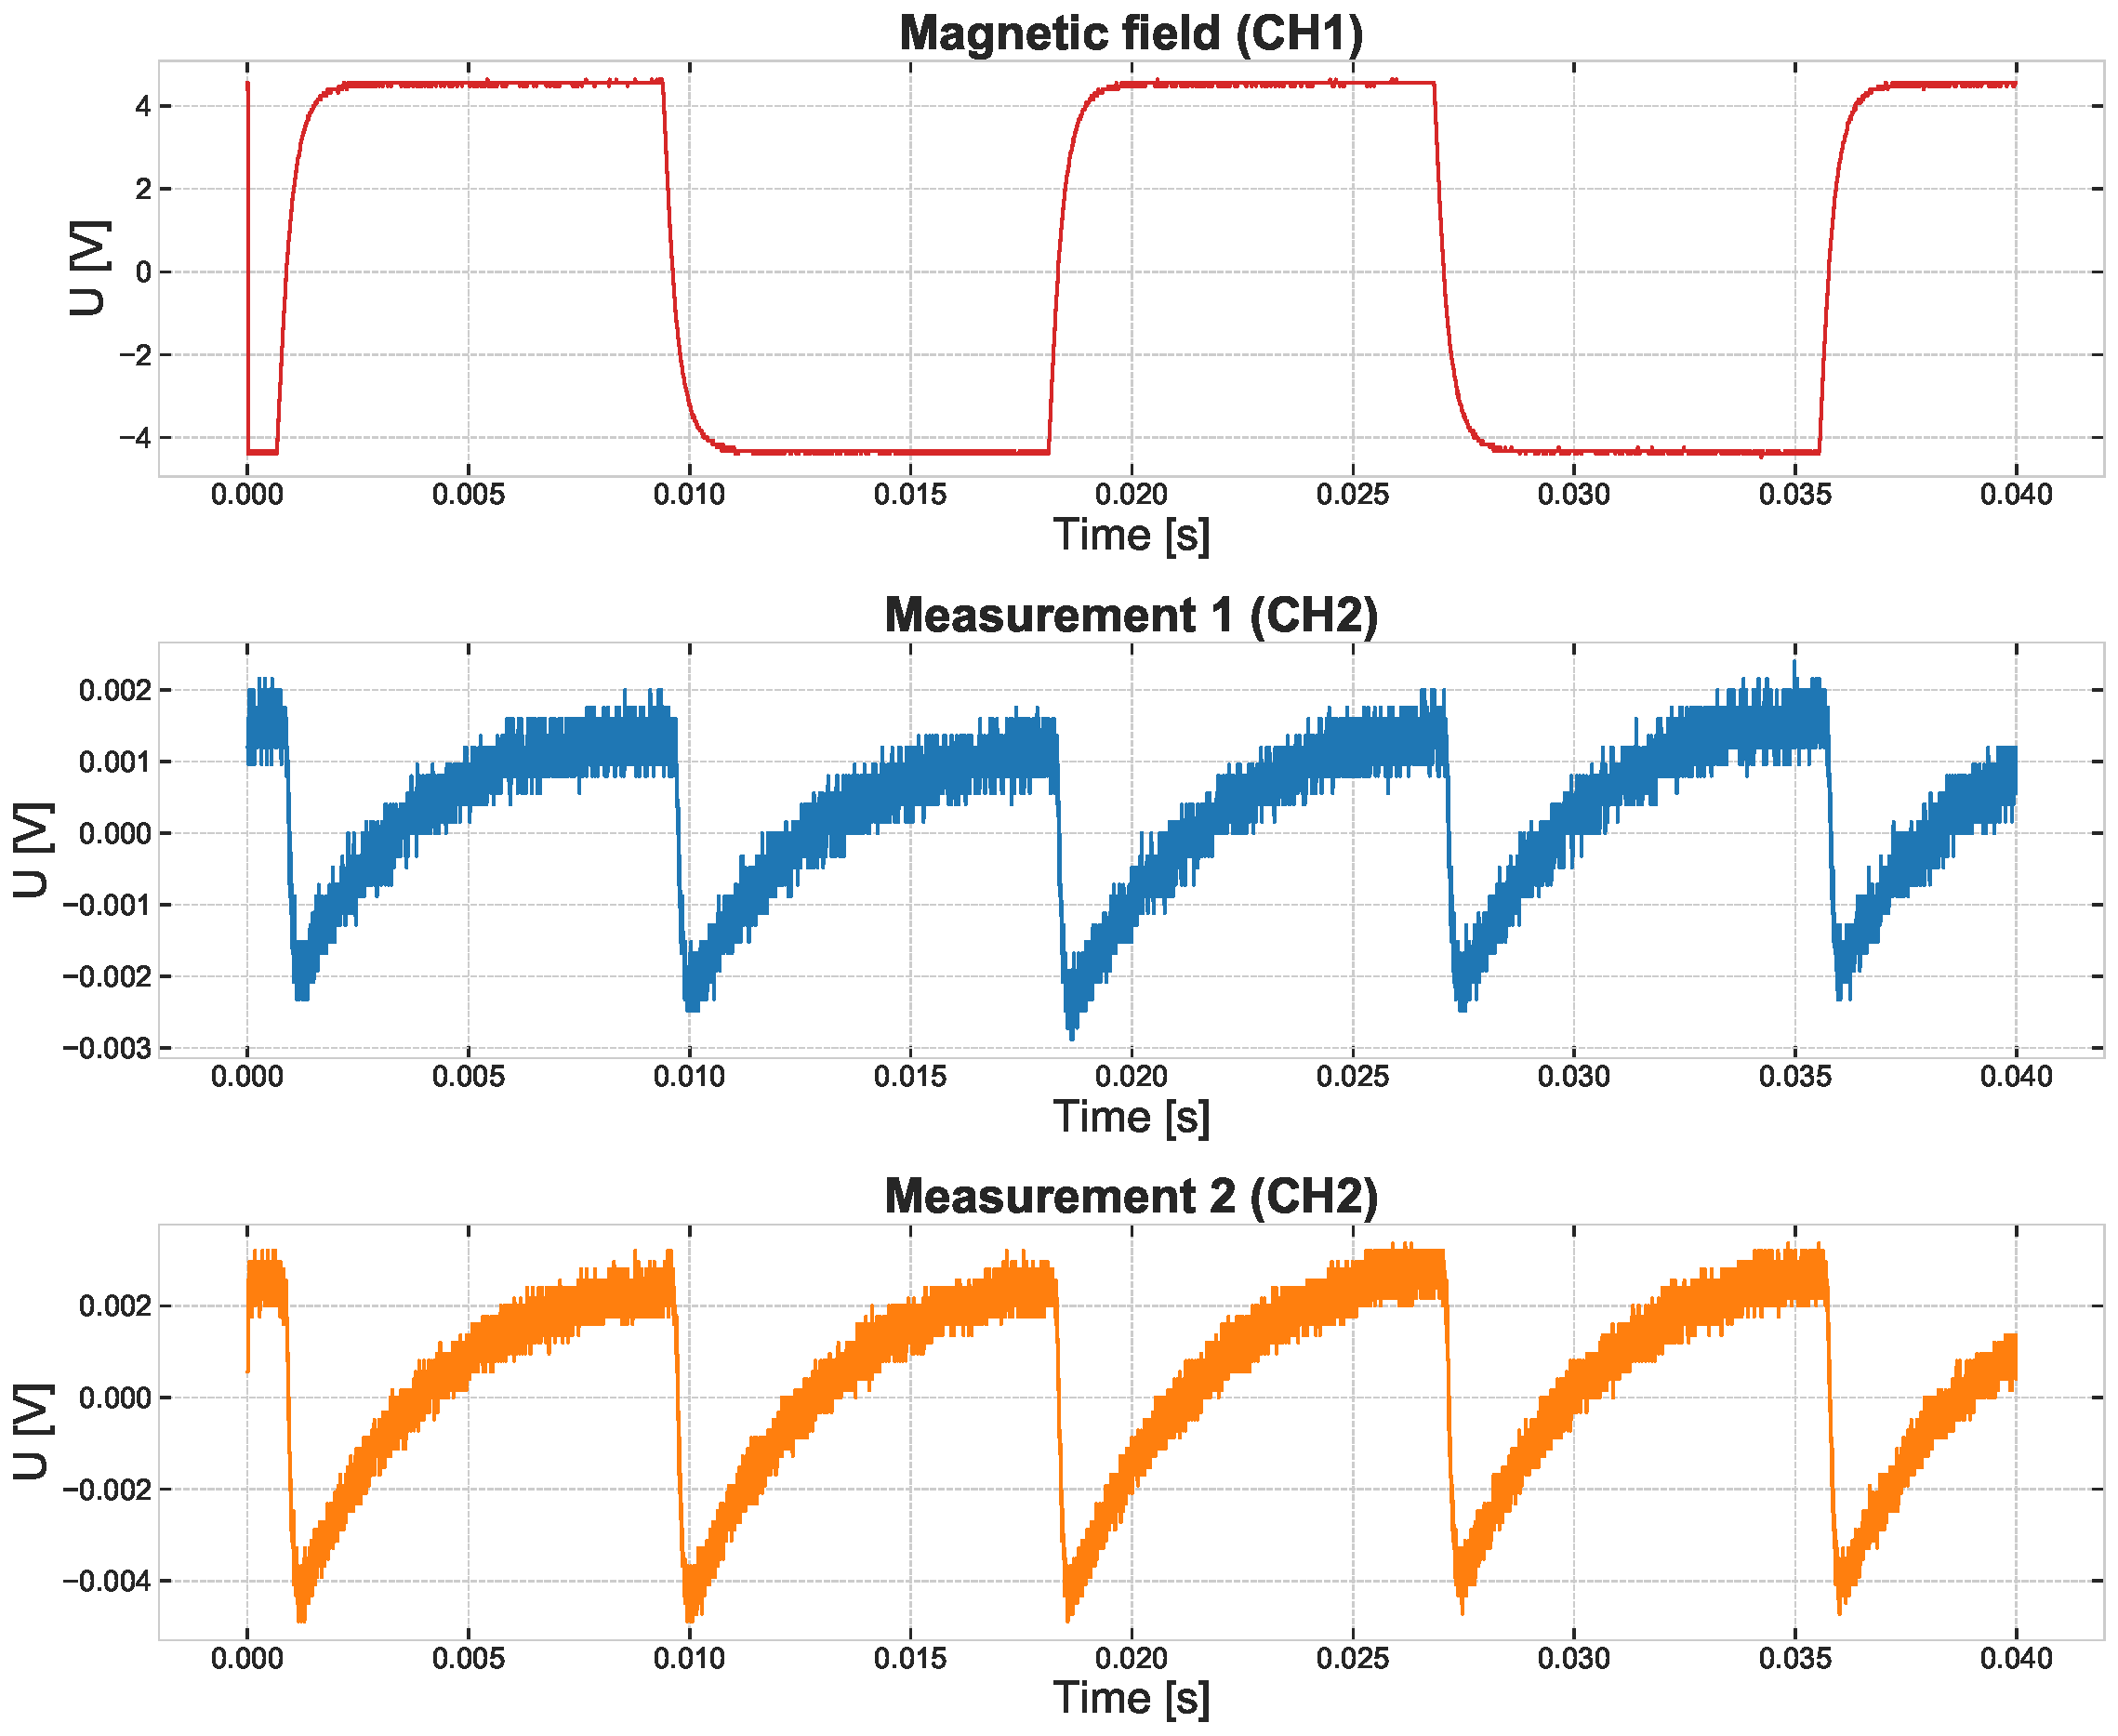
\includegraphics[width=\textwidth]{images/tau.pdf}
    \captionof{figure}{A $\tau$ időállandó meghatározásához az ábra első képén is látható, négyszög alakú jelet vezettünk a Helmholtz-tekercsekbe. A kísérleti összeállítás kimenetén egy fotodióda helyezkedett el, mely a mintán áthaladó és kijövő fény intenzitását volt képes mérni. A kimeneti jelet két időpontban is megmértük, mely felvett jelek az ábra középső és alsó képein láthatóak.} \label{fig:1}
\end{center}
\begin{center}
    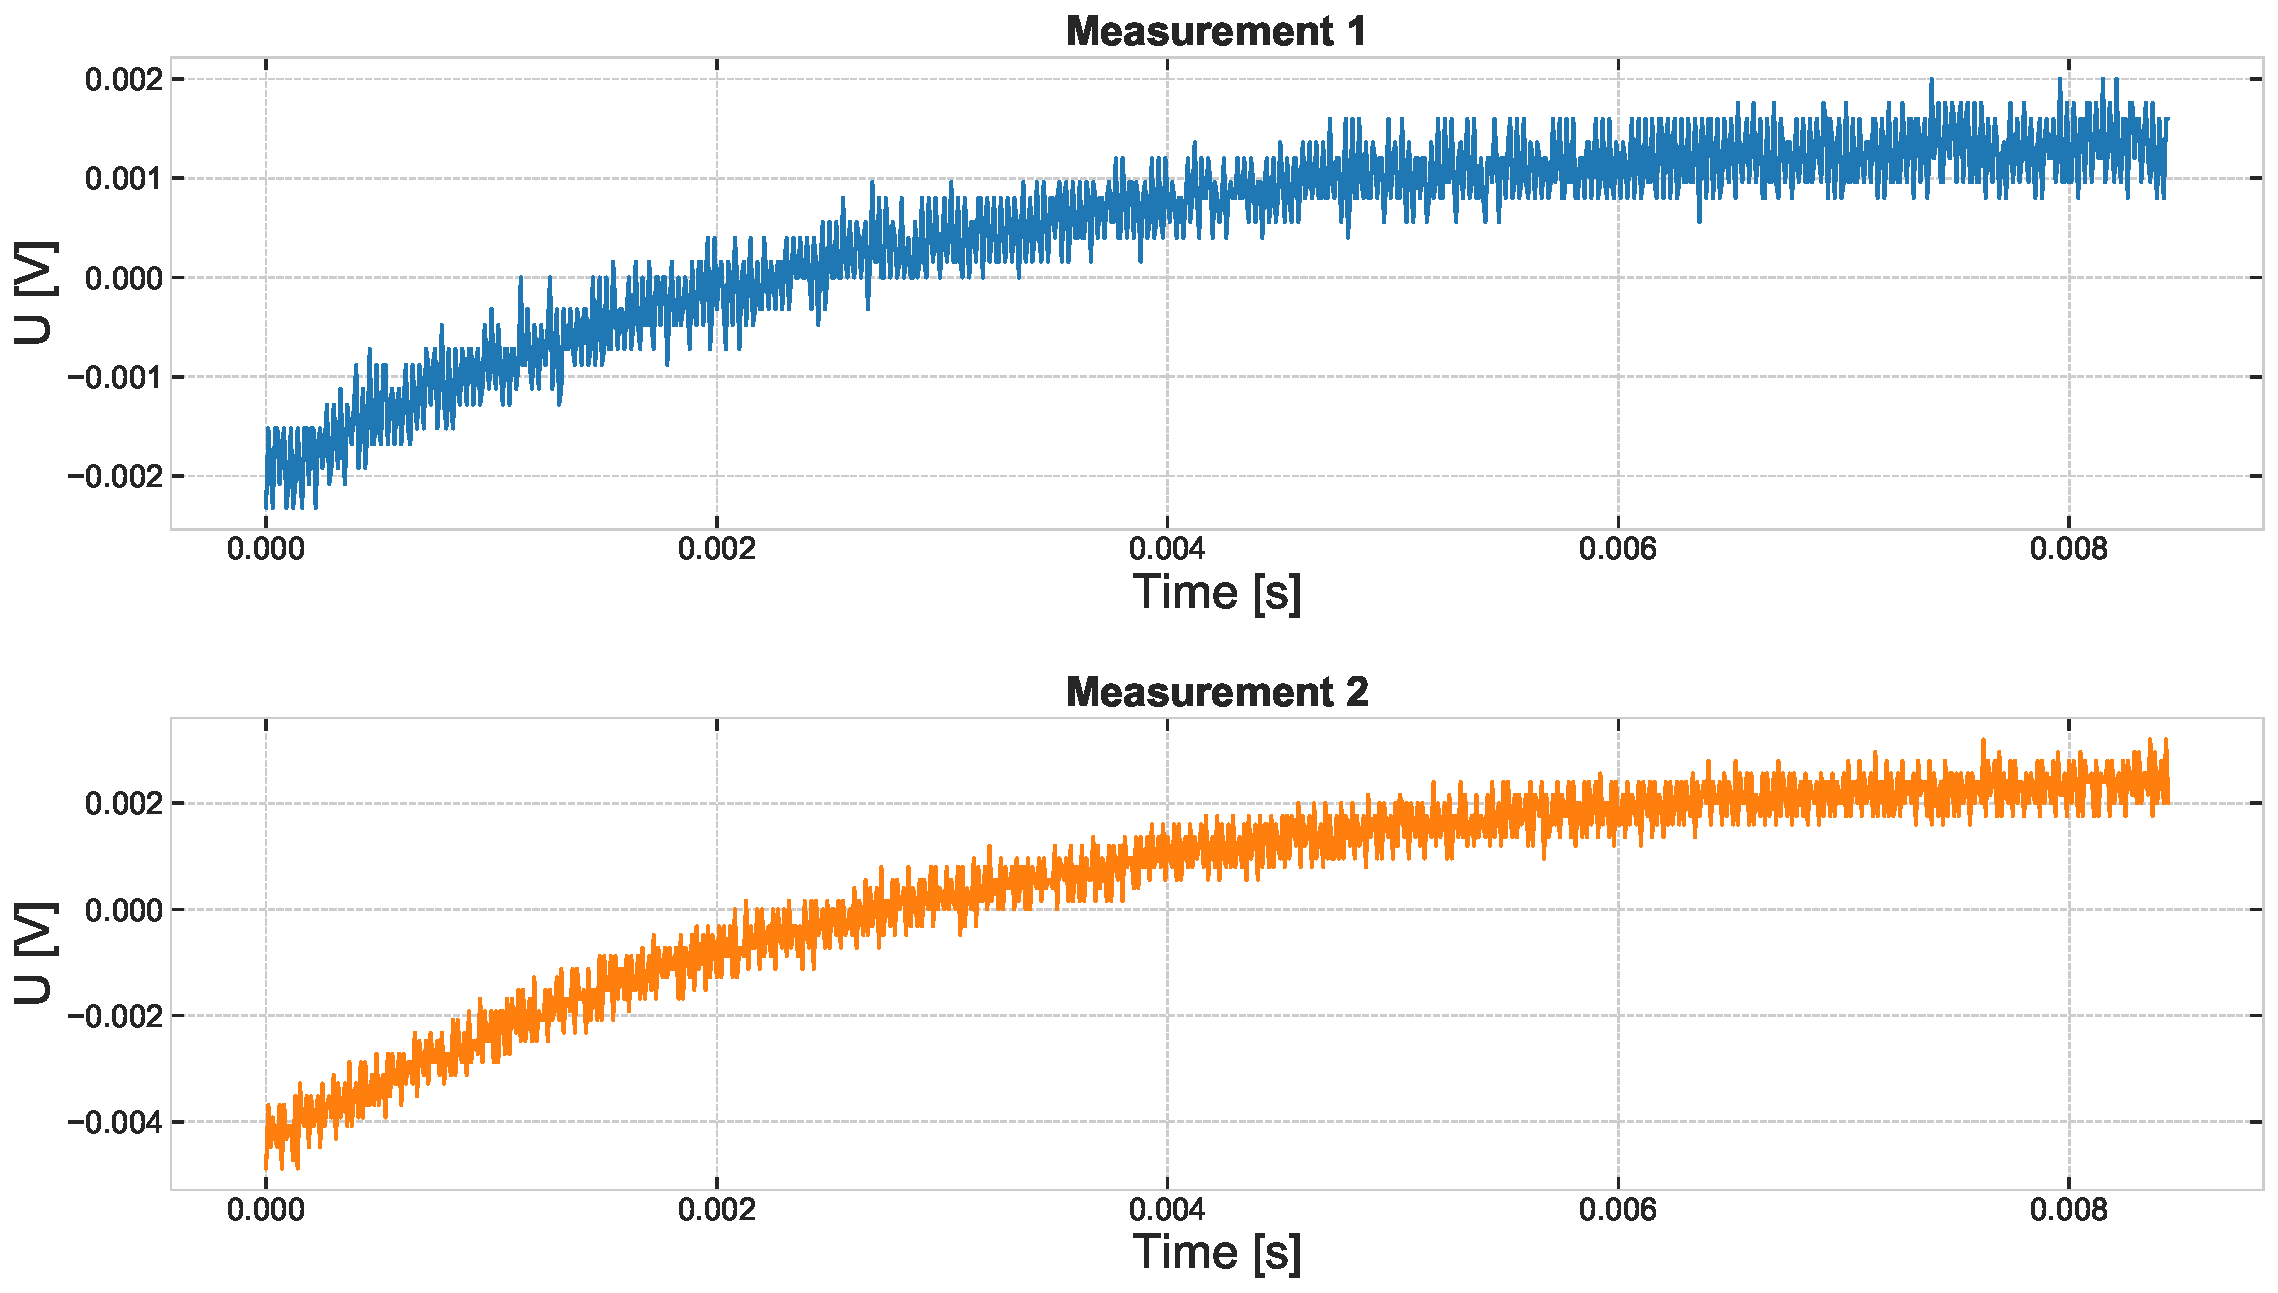
\includegraphics[width=\textwidth]{images/tau_sliced.pdf}
    \captionof{figure}{A $\tau$ mérése során felvett két jel $1$-$1$ kiemelt periódusának felfutó éle. A jelek kezdőpontja a $t=0$-ba van eltolva.} \label{fig:2}
\end{center}
\vspace*{\fill}
\newpage
\topskip0pt
\vspace*{\fill}
\begin{center}
    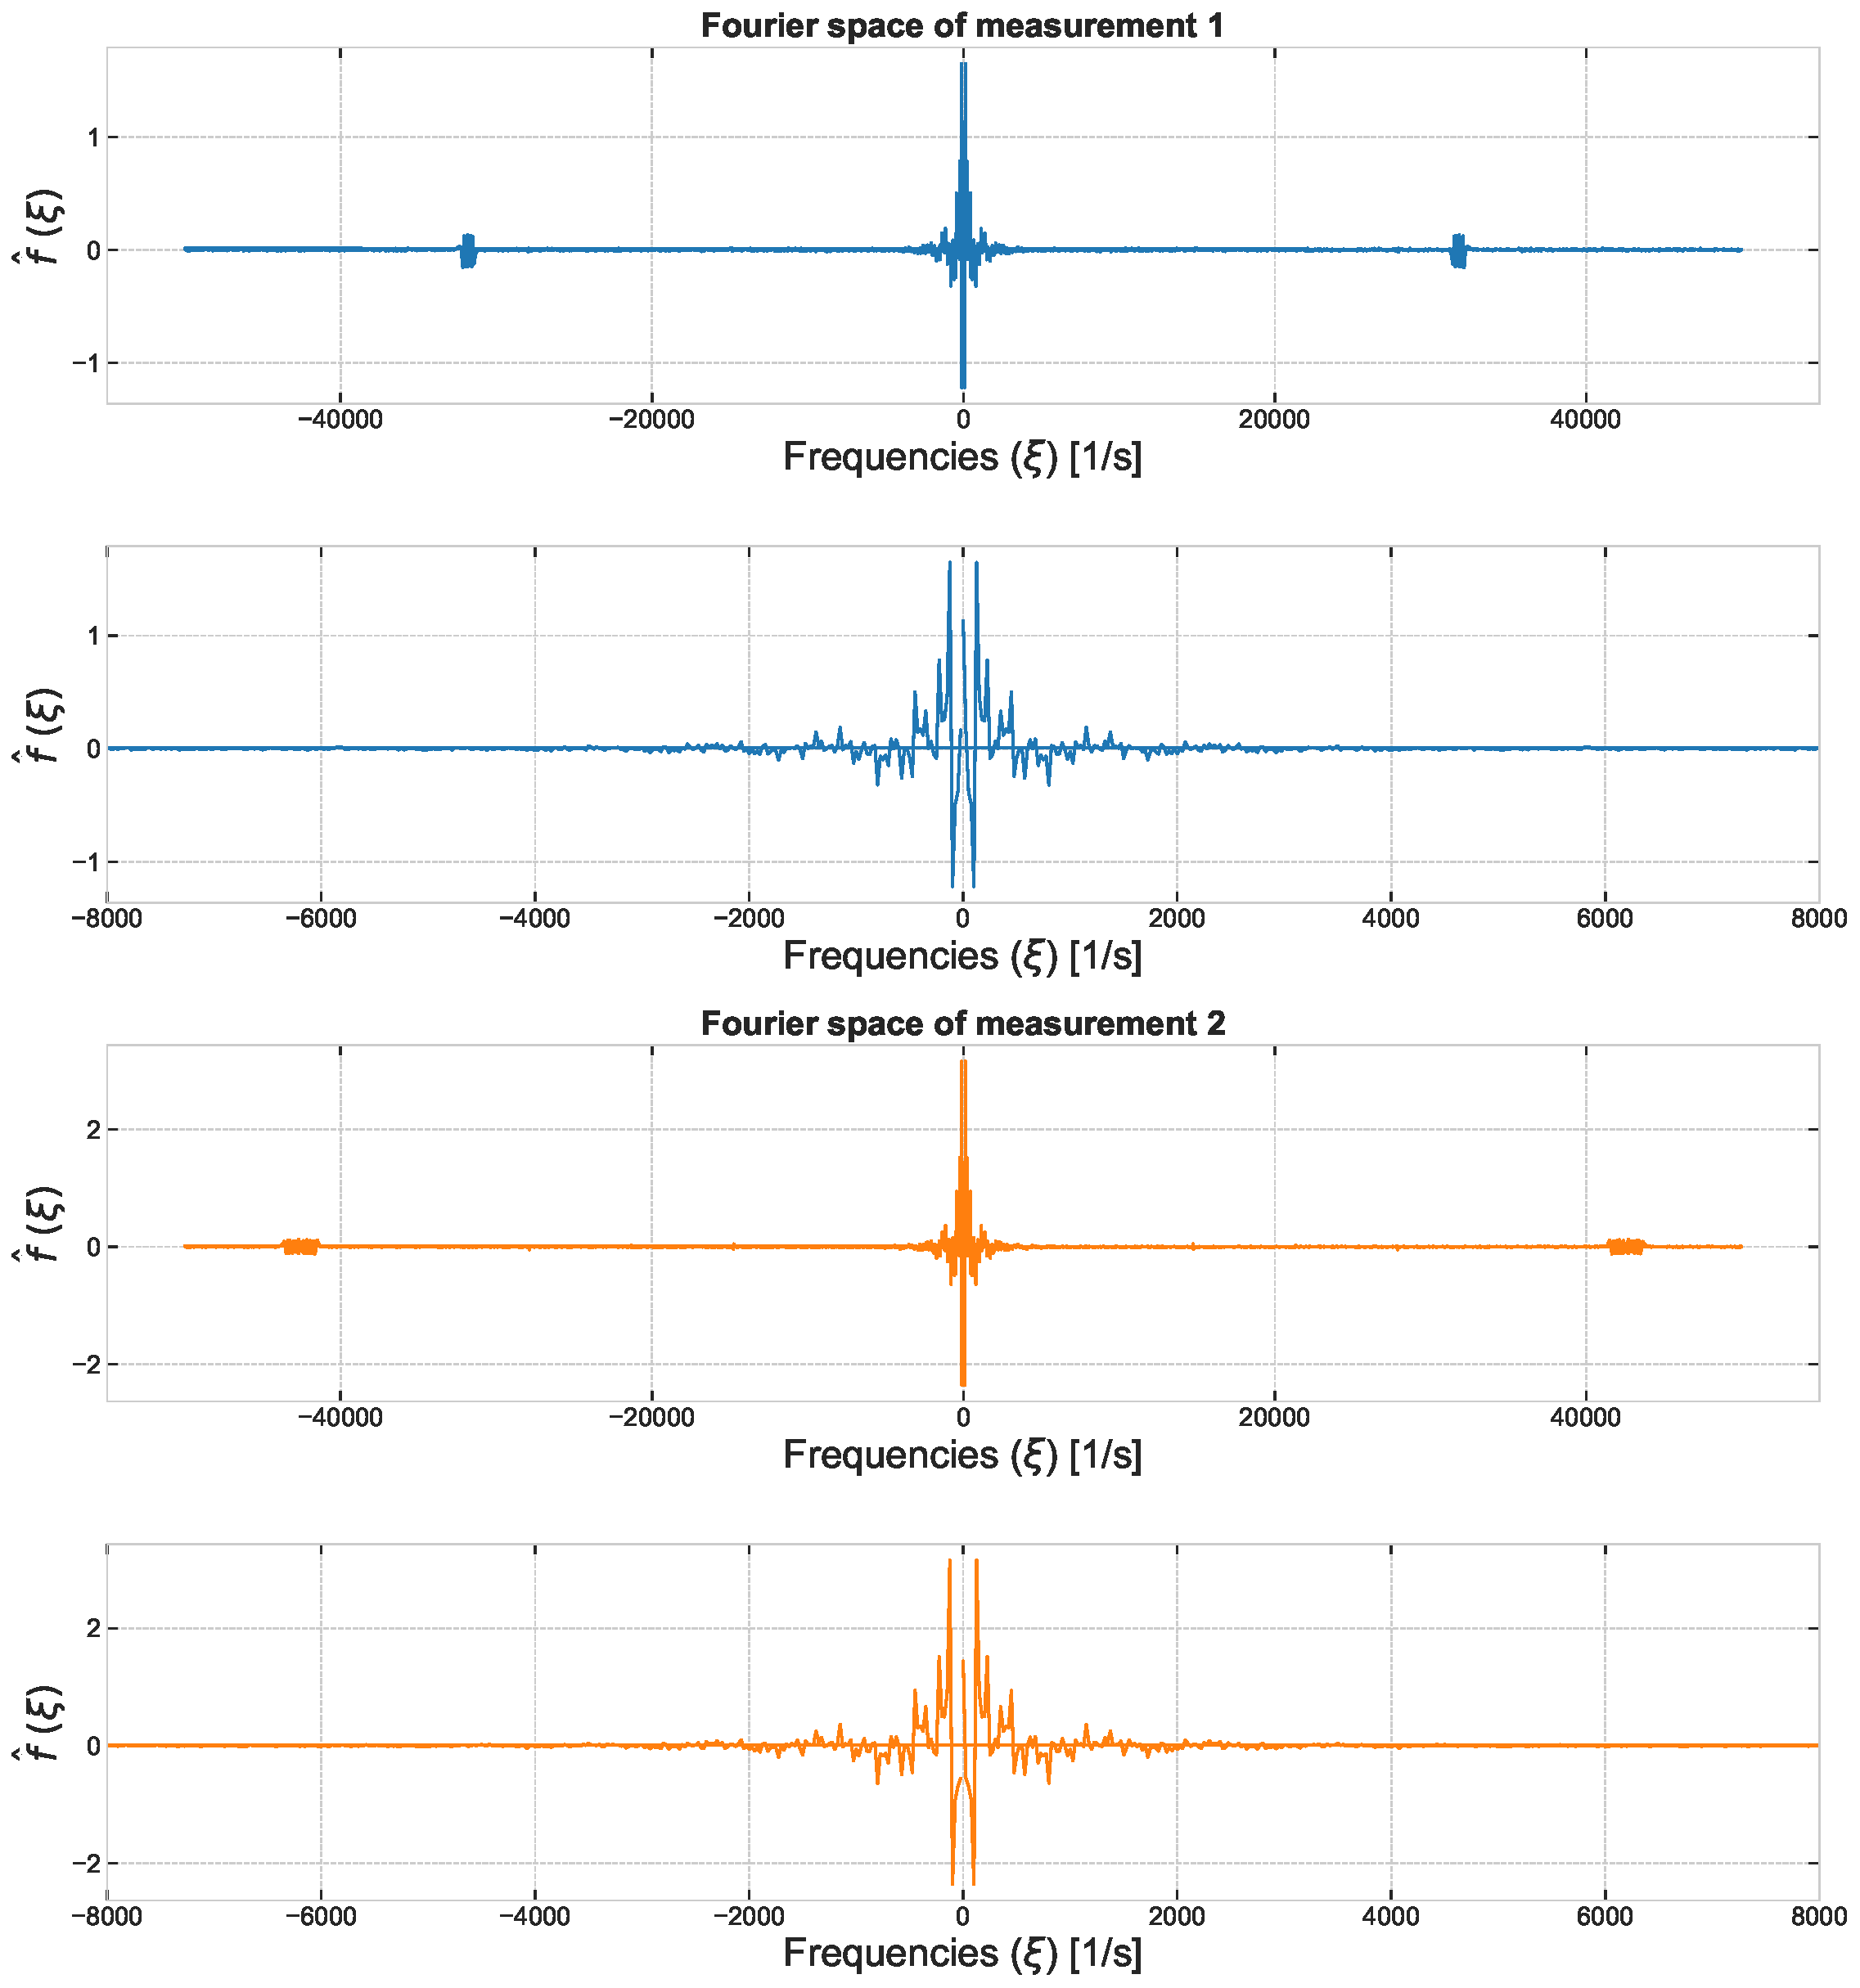
\includegraphics[width=\textwidth]{images/tau_fourier.pdf}
    \captionof{figure}{A $\tau$ mérése során felvett két jel Fourier-térben ábrázolva. Az 1. és 3. képen a jelek teljes frekvenciatere látható, míg a 2. és 4. képen csak a $8000$ Hz alatti frekvenciák szerepelnek.} \label{fig:3}
\end{center}
\vspace*{\fill}
\newpage
\topskip0pt
\vspace*{\fill}
\begin{center}
    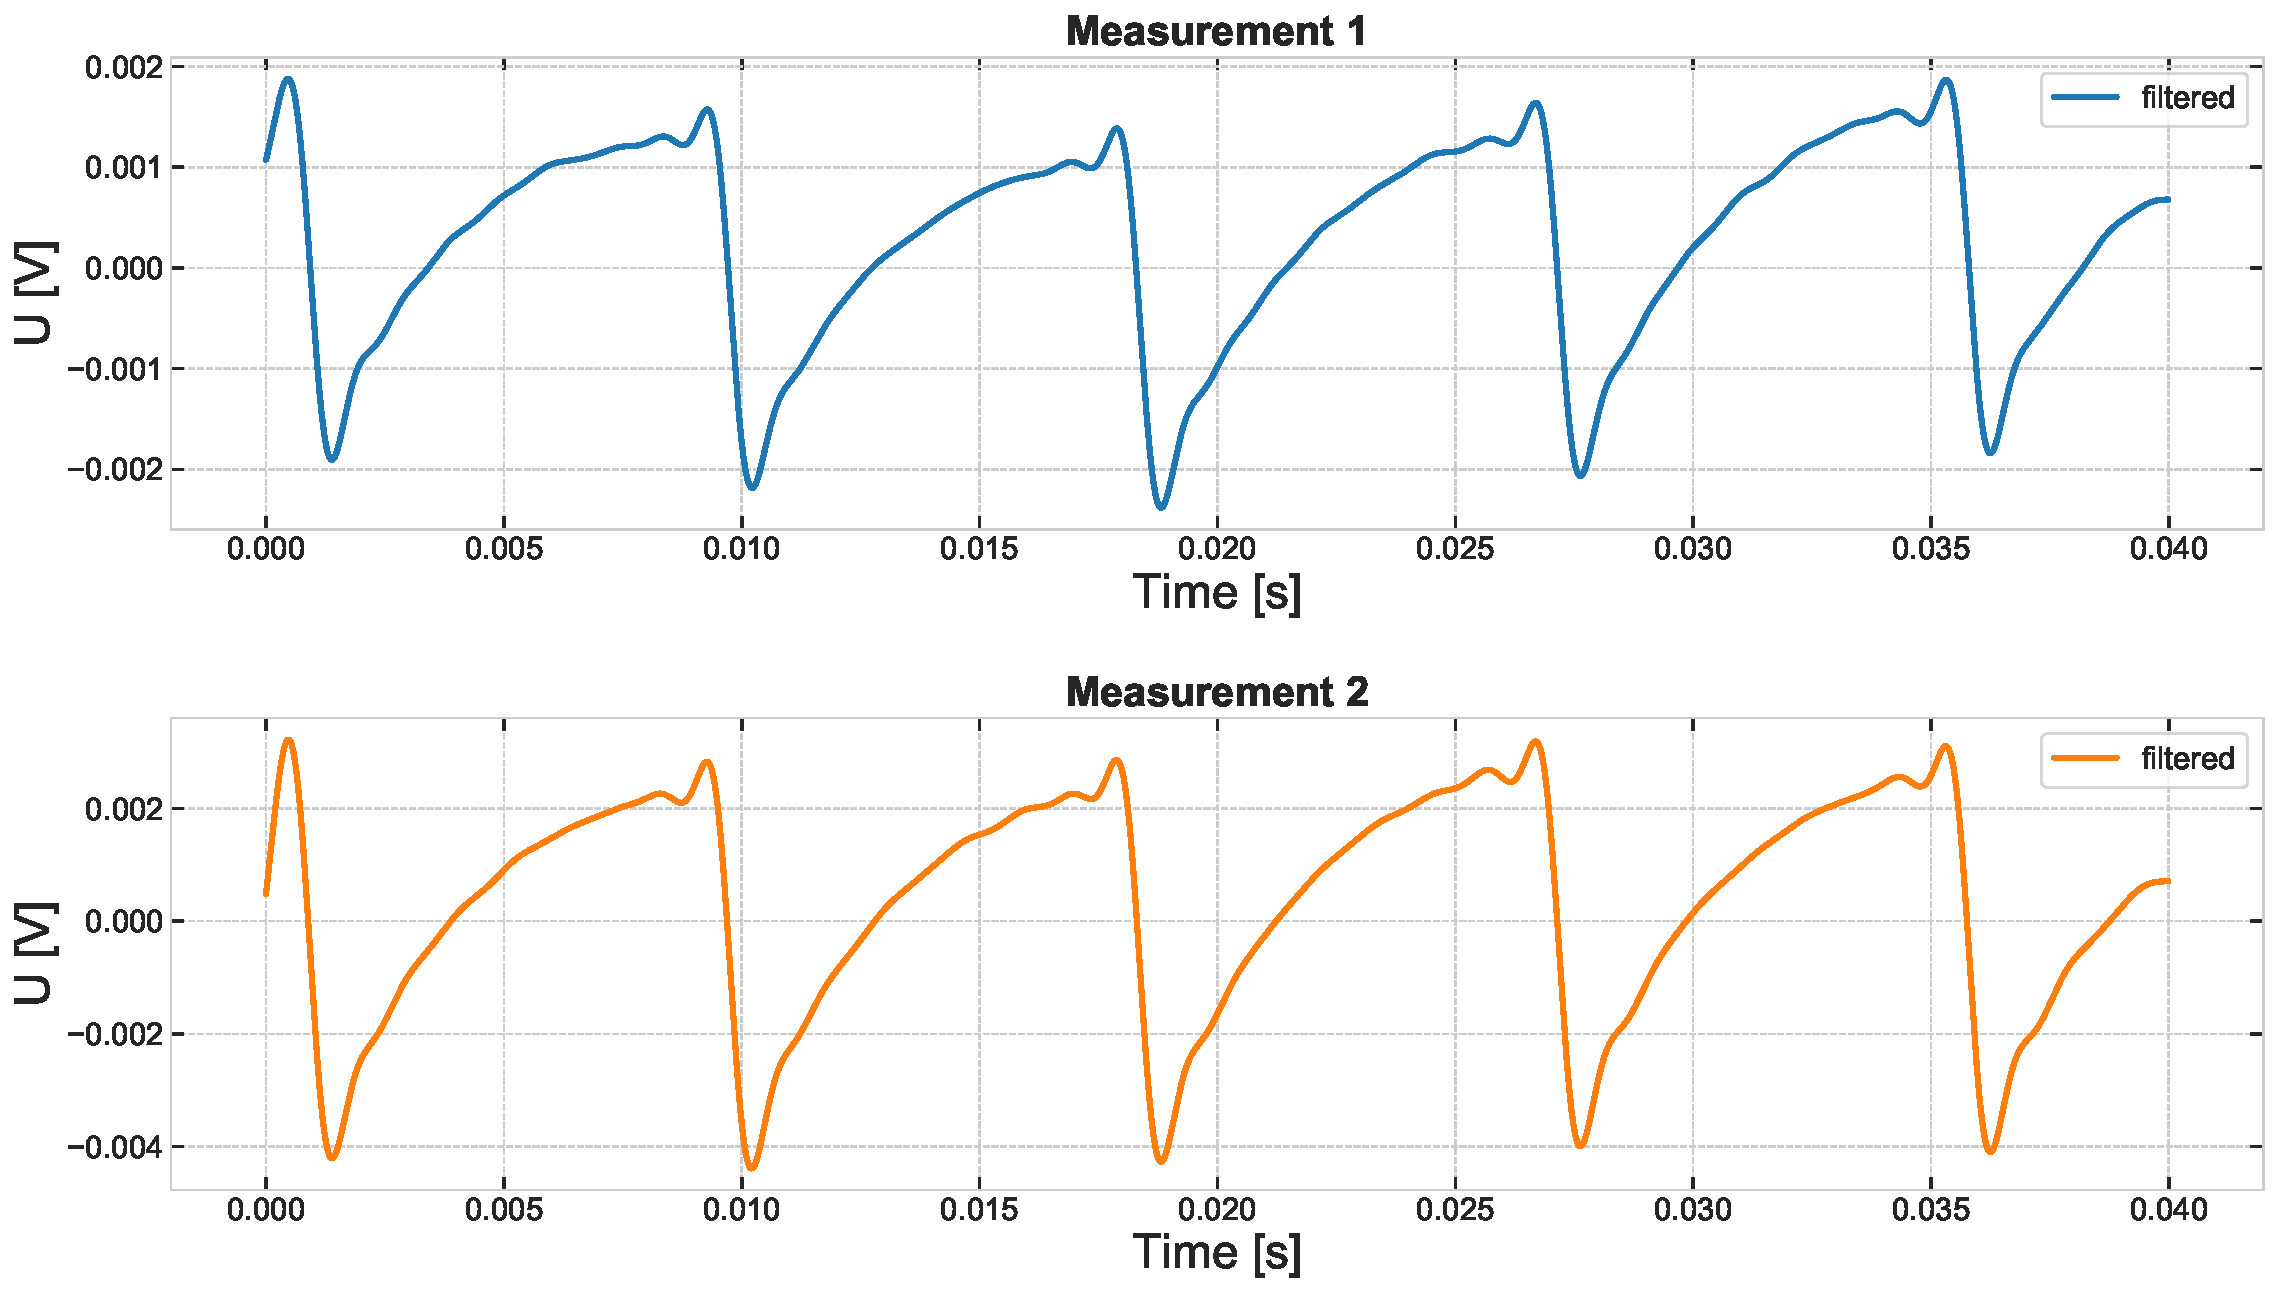
\includegraphics[width=\textwidth]{images/tau_butterworth.pdf}
    \captionof{figure}{A $\tau$ mérése során felvett két jel egy $f_{C} = 1000$ Hz levágási frekvenciával rendelkező aluláteresztő szűrön átengedve.} \label{fig:4}
\end{center}
\begin{center}
    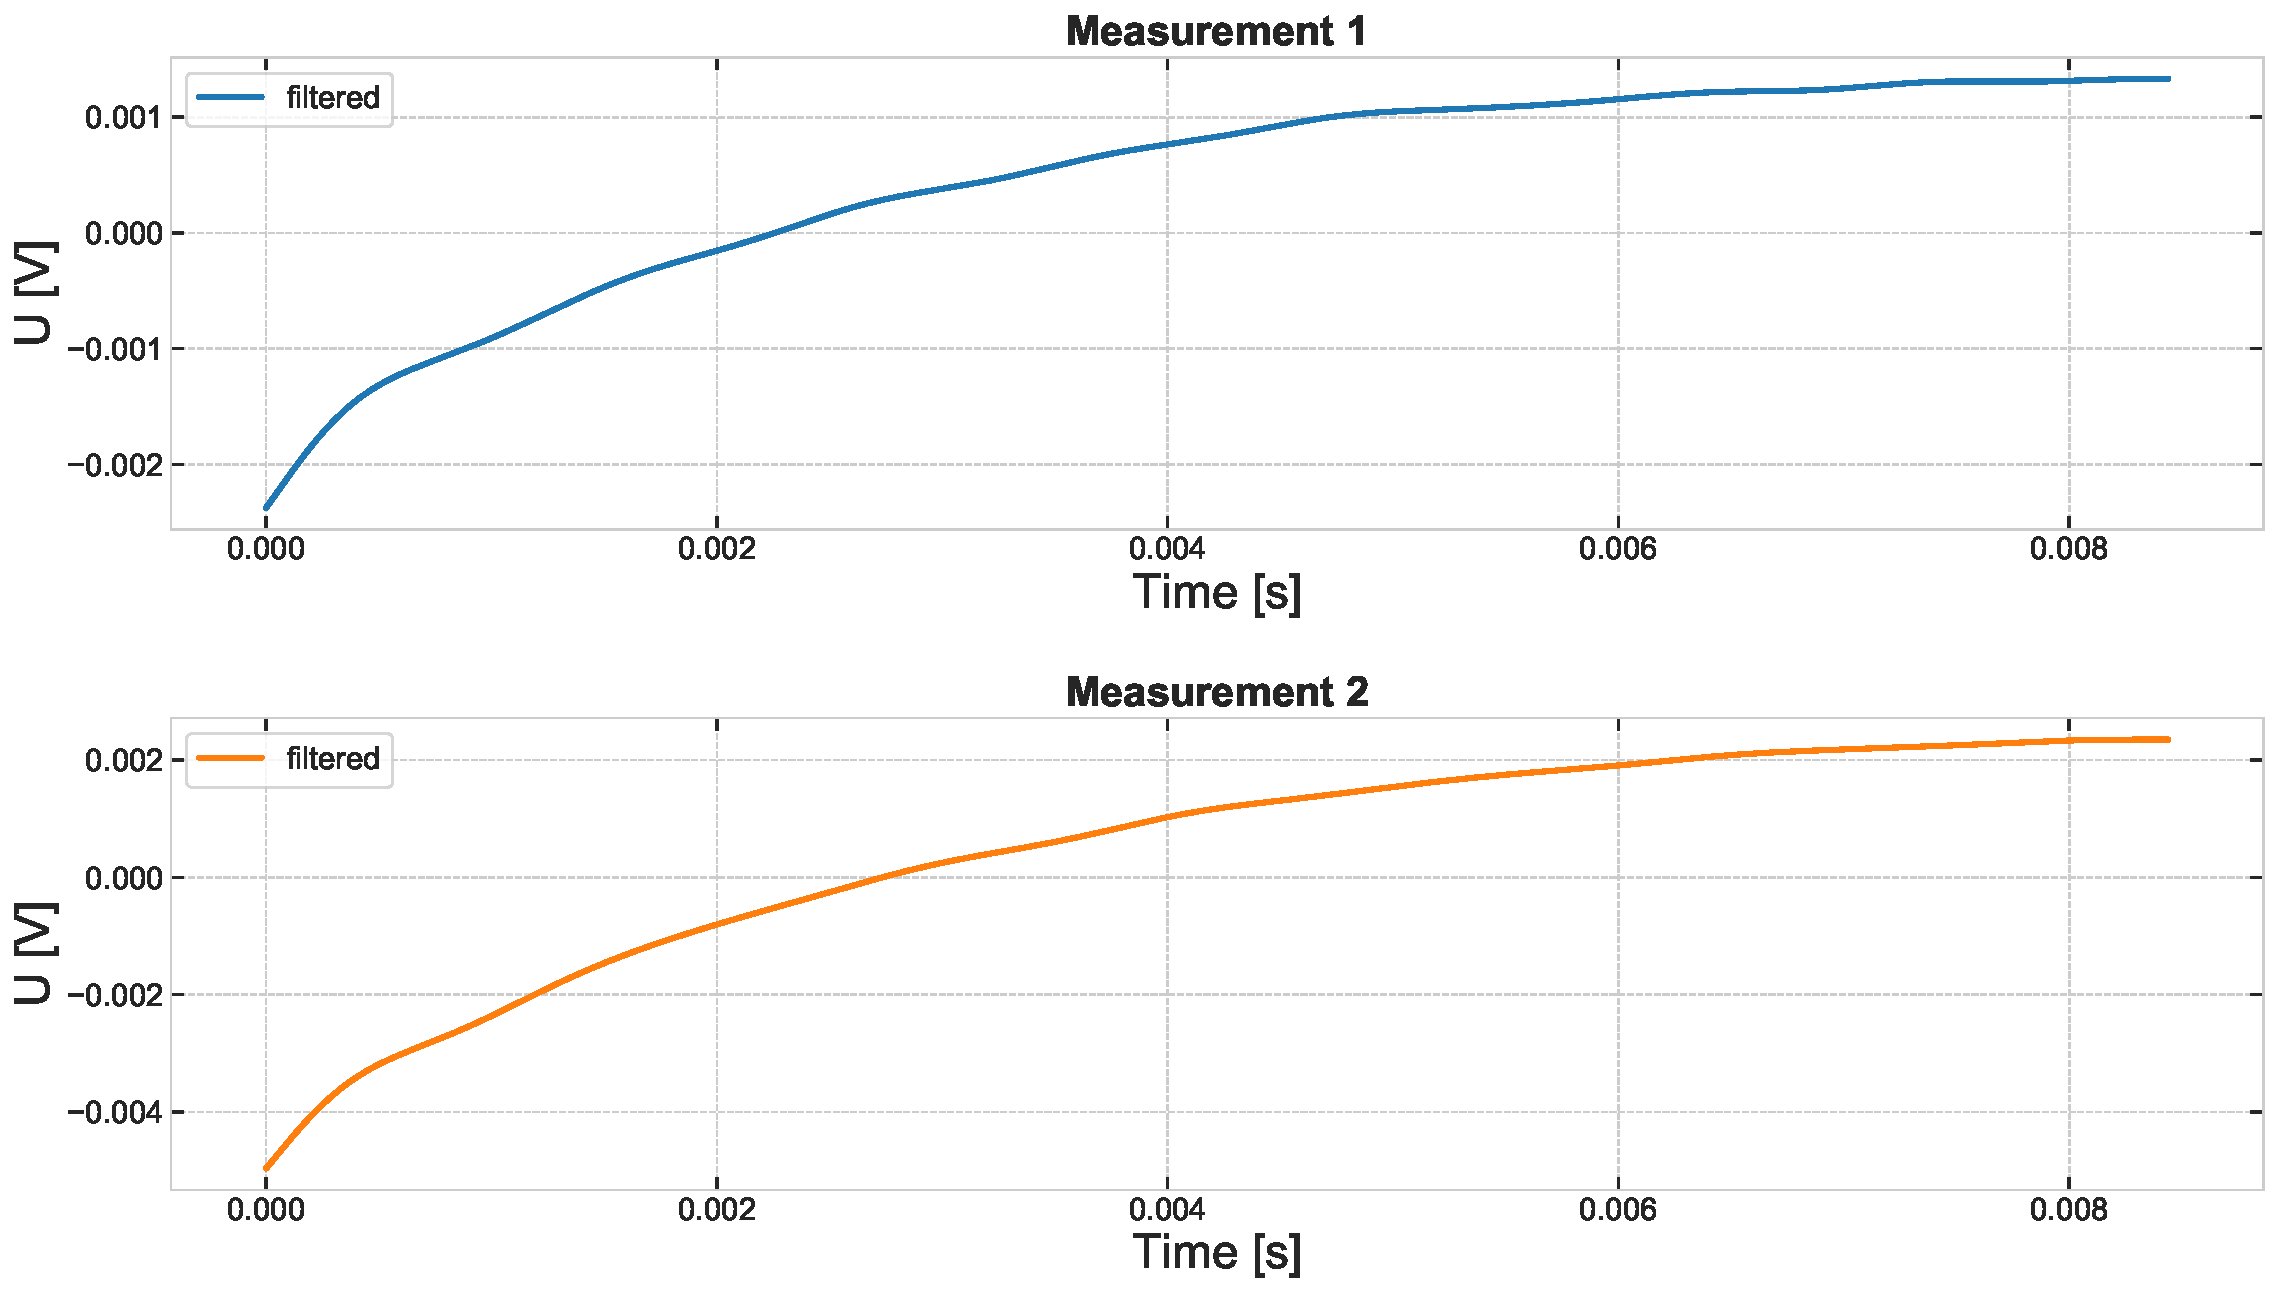
\includegraphics[width=\textwidth]{images/tau_sliced_butterworth.pdf}
    \captionof{figure}{A $\tau$ mérése során felvett két jel egy $f_{C} = 1000$ Hz levágási frekvenciával rendelkező aluláteresztő szűrön átengedve. Az ábrán a jelek $1$-$1$ kiemelt periódusának felfutó élei láthatóak. A jelek kezdőpontja a $t=0$-ba van eltolva.} \label{fig:5}
\end{center}
\vspace*{\fill}
\newpage
\topskip0pt
\vspace*{\fill}
\begin{center}
    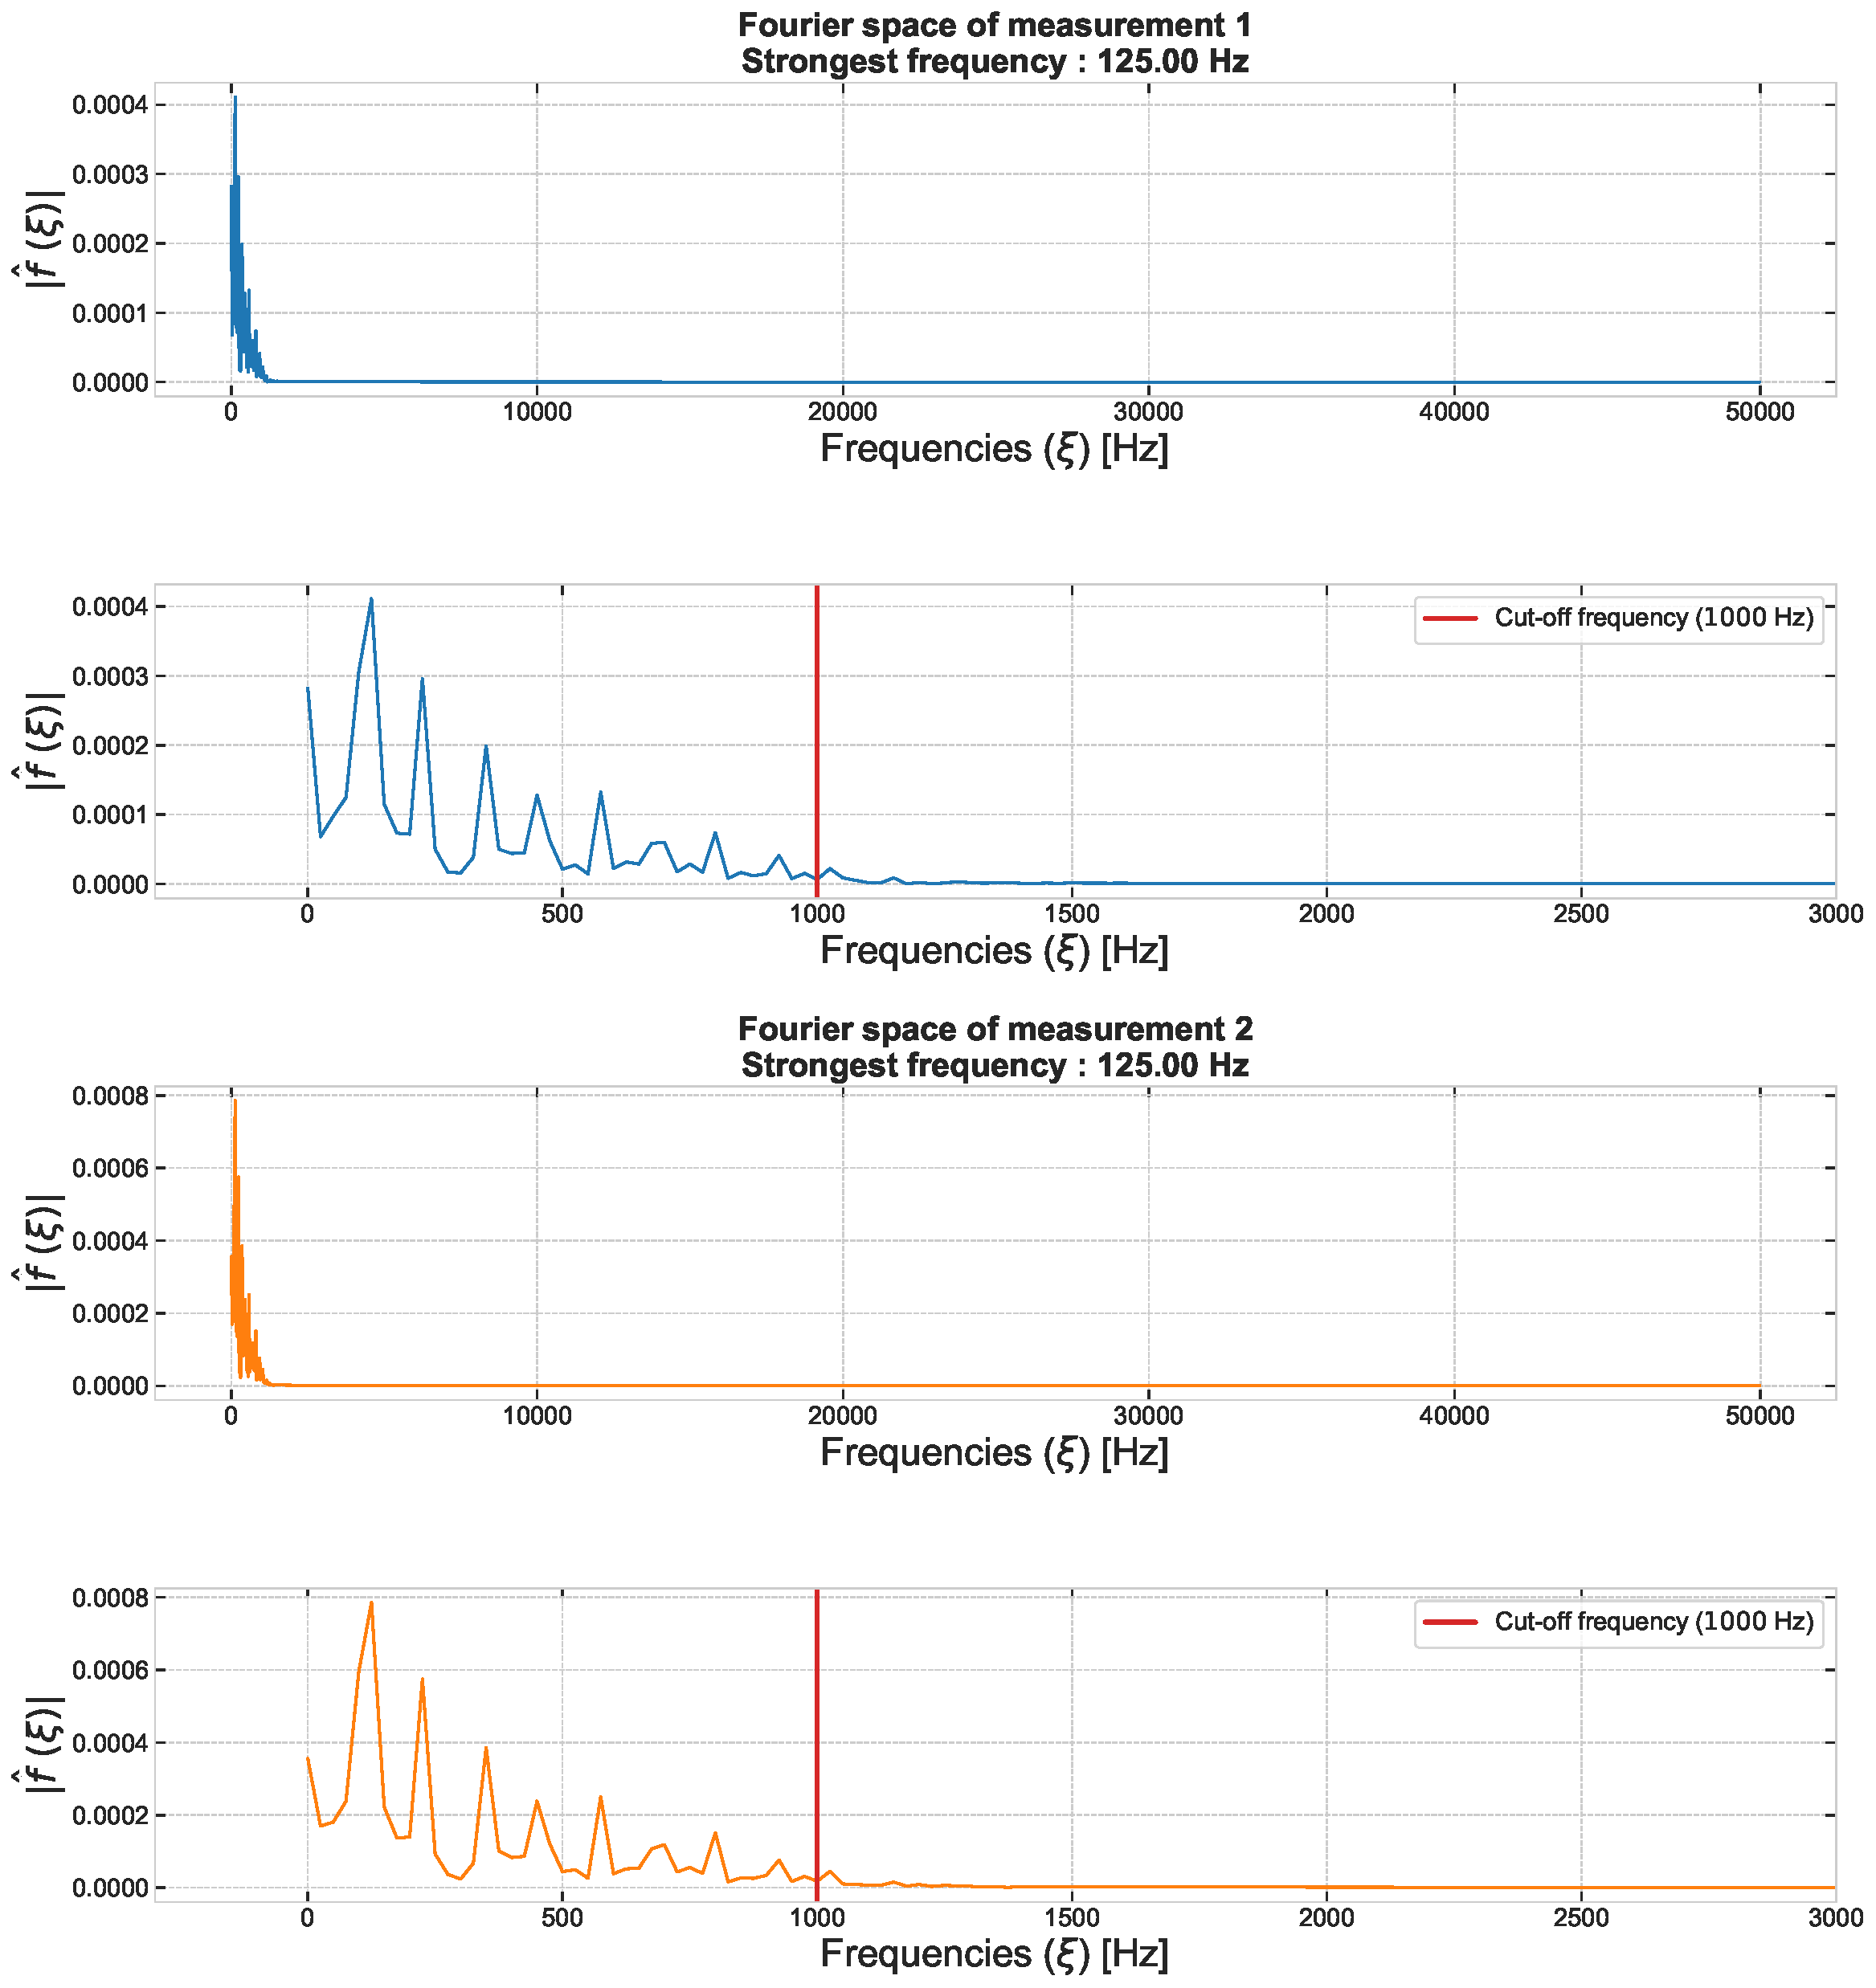
\includegraphics[width=\textwidth]{images/tau_butterworth_fourier.pdf}
    \captionof{figure}{Az aluláteresztő szűrön átengedett jelalak Fourier-térben ábrázolva. A függőleges vörös vonal a szűrő levágási frekvenciáját jelzi. Az 1. és 3. képen a jelek teljes frekvenciatere látható, míg a 2. és 4. képen csak a szűrő $f_{C}$ levágási frekvenciájának háromszorosánál kisebb értékek szerepelnek.} \label{fig:6}
\end{center}
\vspace*{\fill}
\newpage
\topskip0pt
\vspace*{\fill}
\begin{center}
    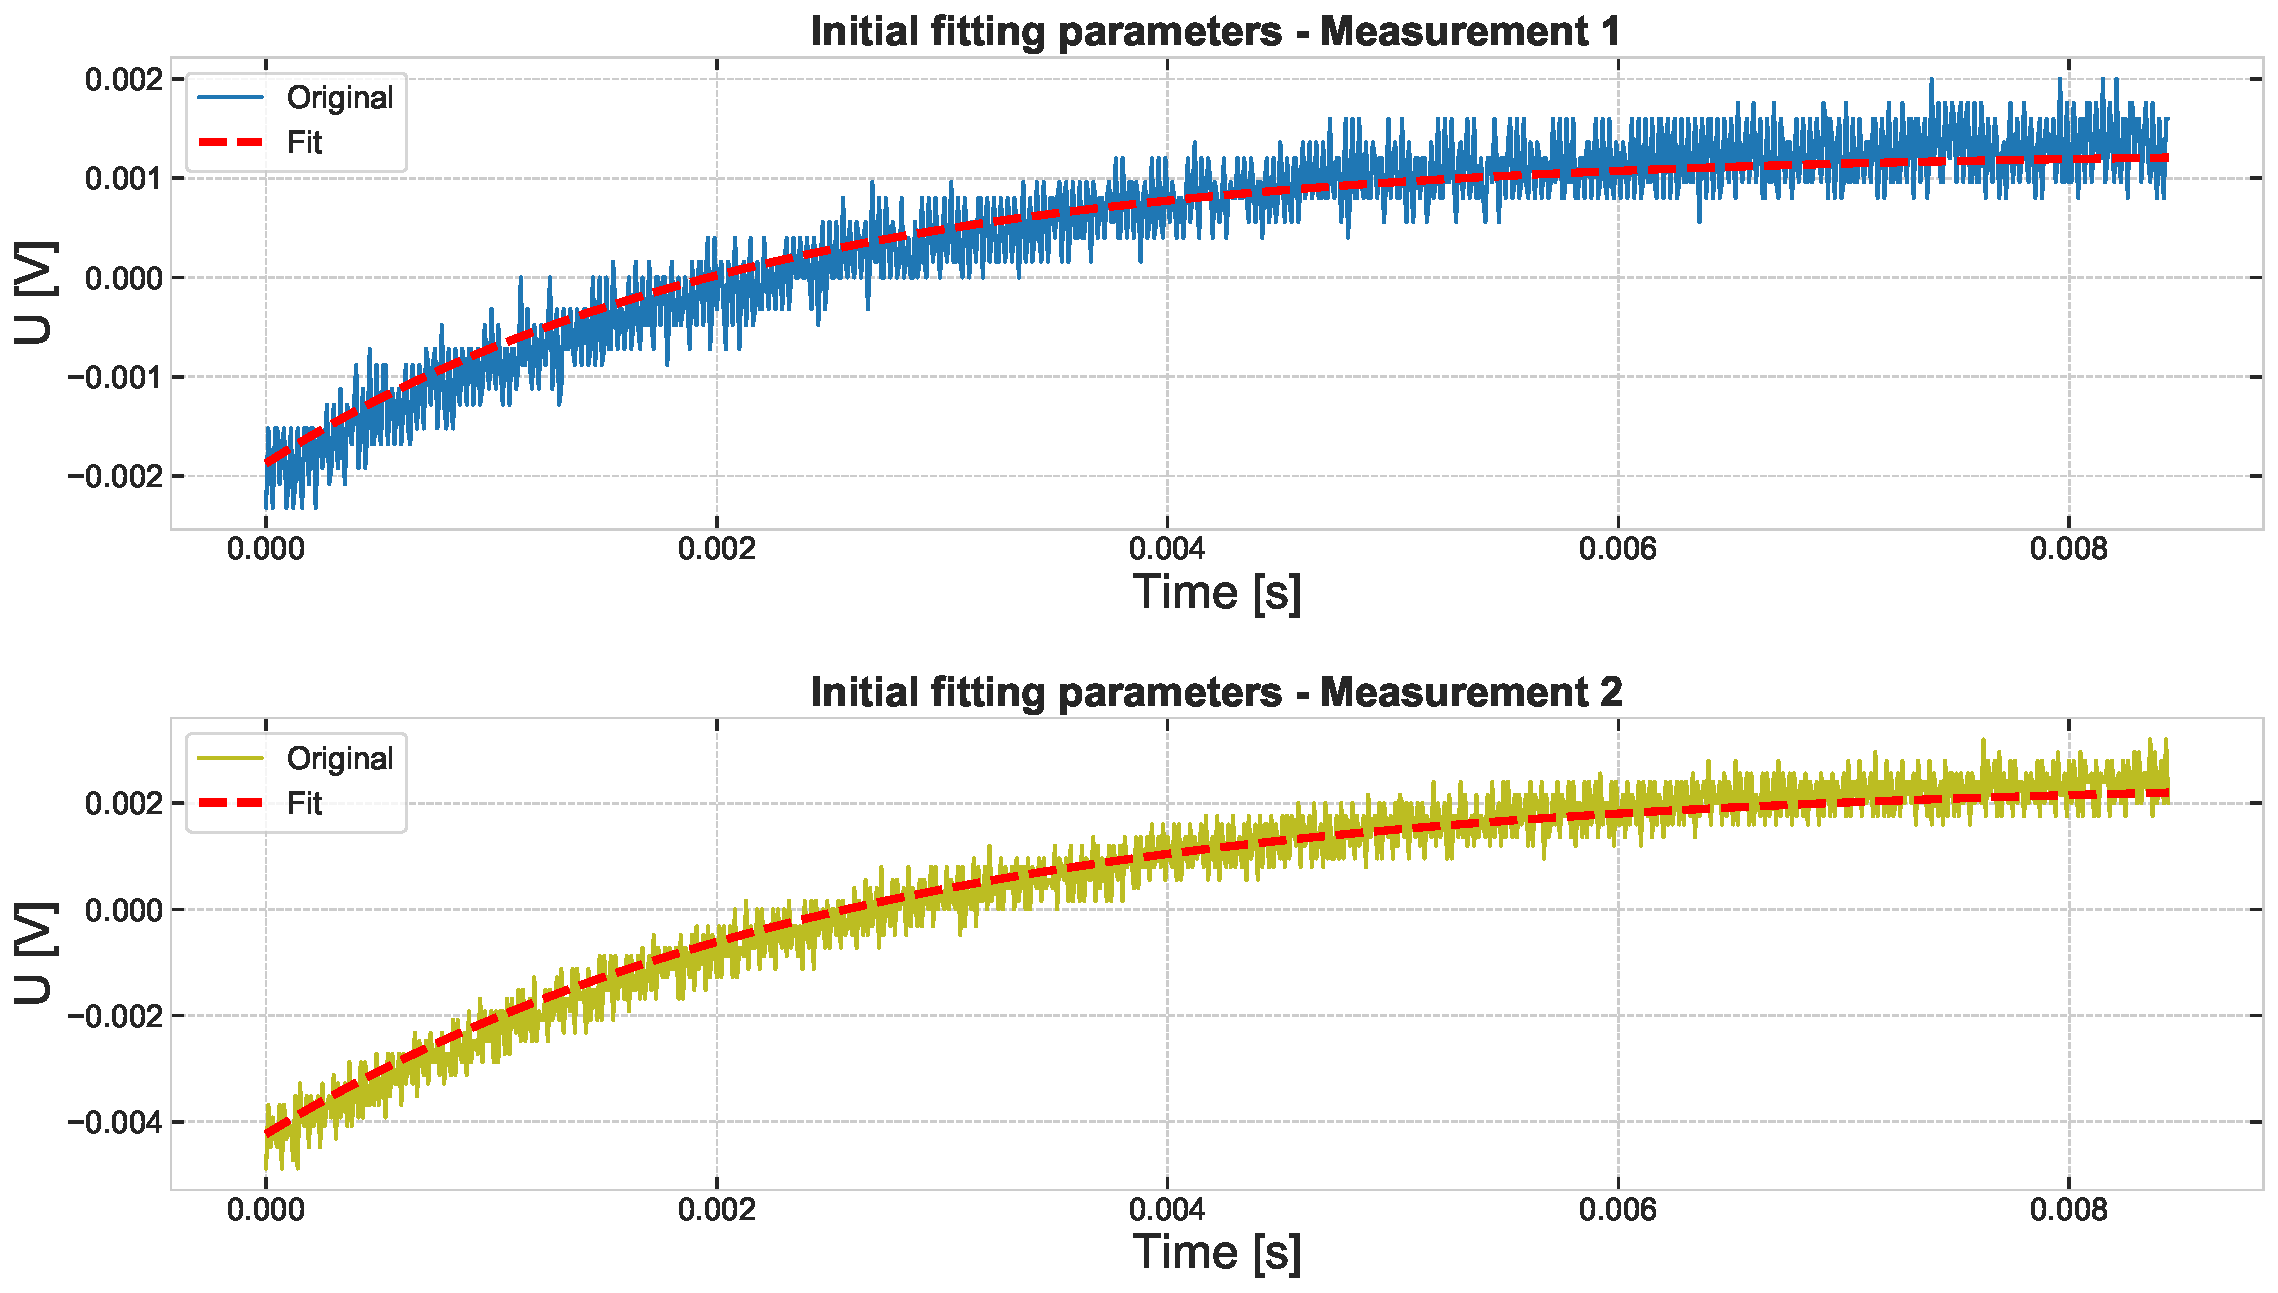
\includegraphics[width=\textwidth]{images/tau_fitted_initial.pdf}
    \captionof{figure}{A $\tau$ mérése során kapott, szűrés nélküli jelalak egyik felfutó élére illesztett paraméteres görbe az első lépésben becsült együtthatóival ábrázolva.} \label{fig:7}
\end{center}
\begin{center}
    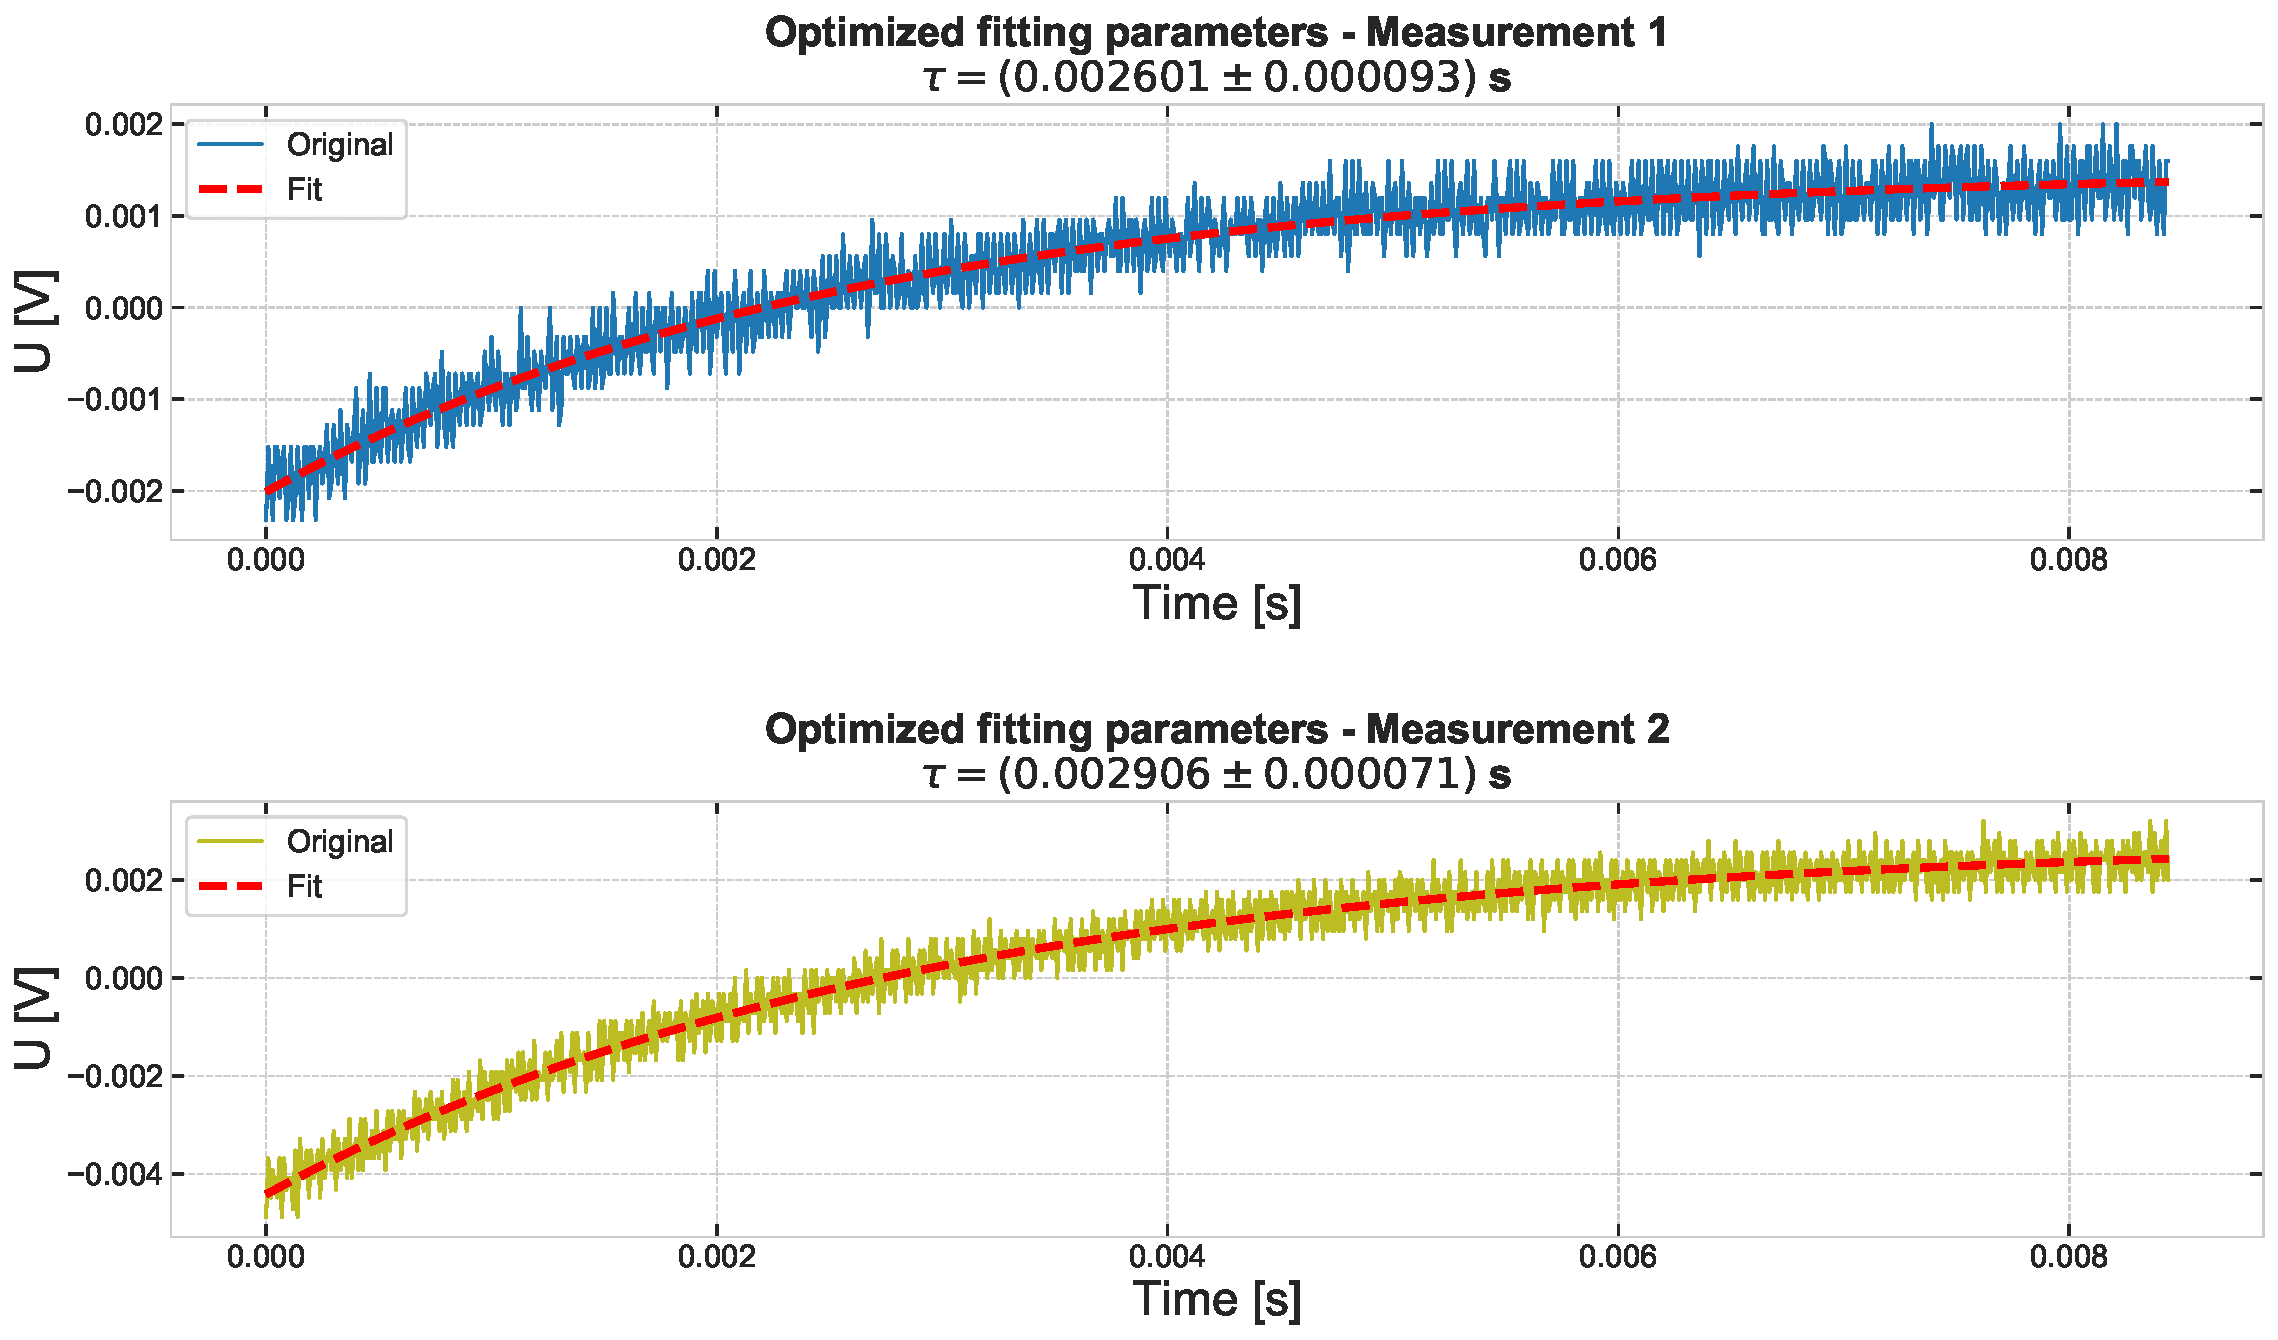
\includegraphics[width=\textwidth]{images/tau_fitted_optimized.pdf}
    \captionof{figure}{A $\tau$ mérése során kapott, szűrés nélküli jelalak egyik felfutó élére illesztett paraméteres görbe a függvényillesztési iterációk után optimalizált együtthatóival ábrázolva.} \label{fig:8}
\end{center}
\vspace*{\fill}
\newpage
\topskip0pt
\vspace*{\fill}
\begin{center}
    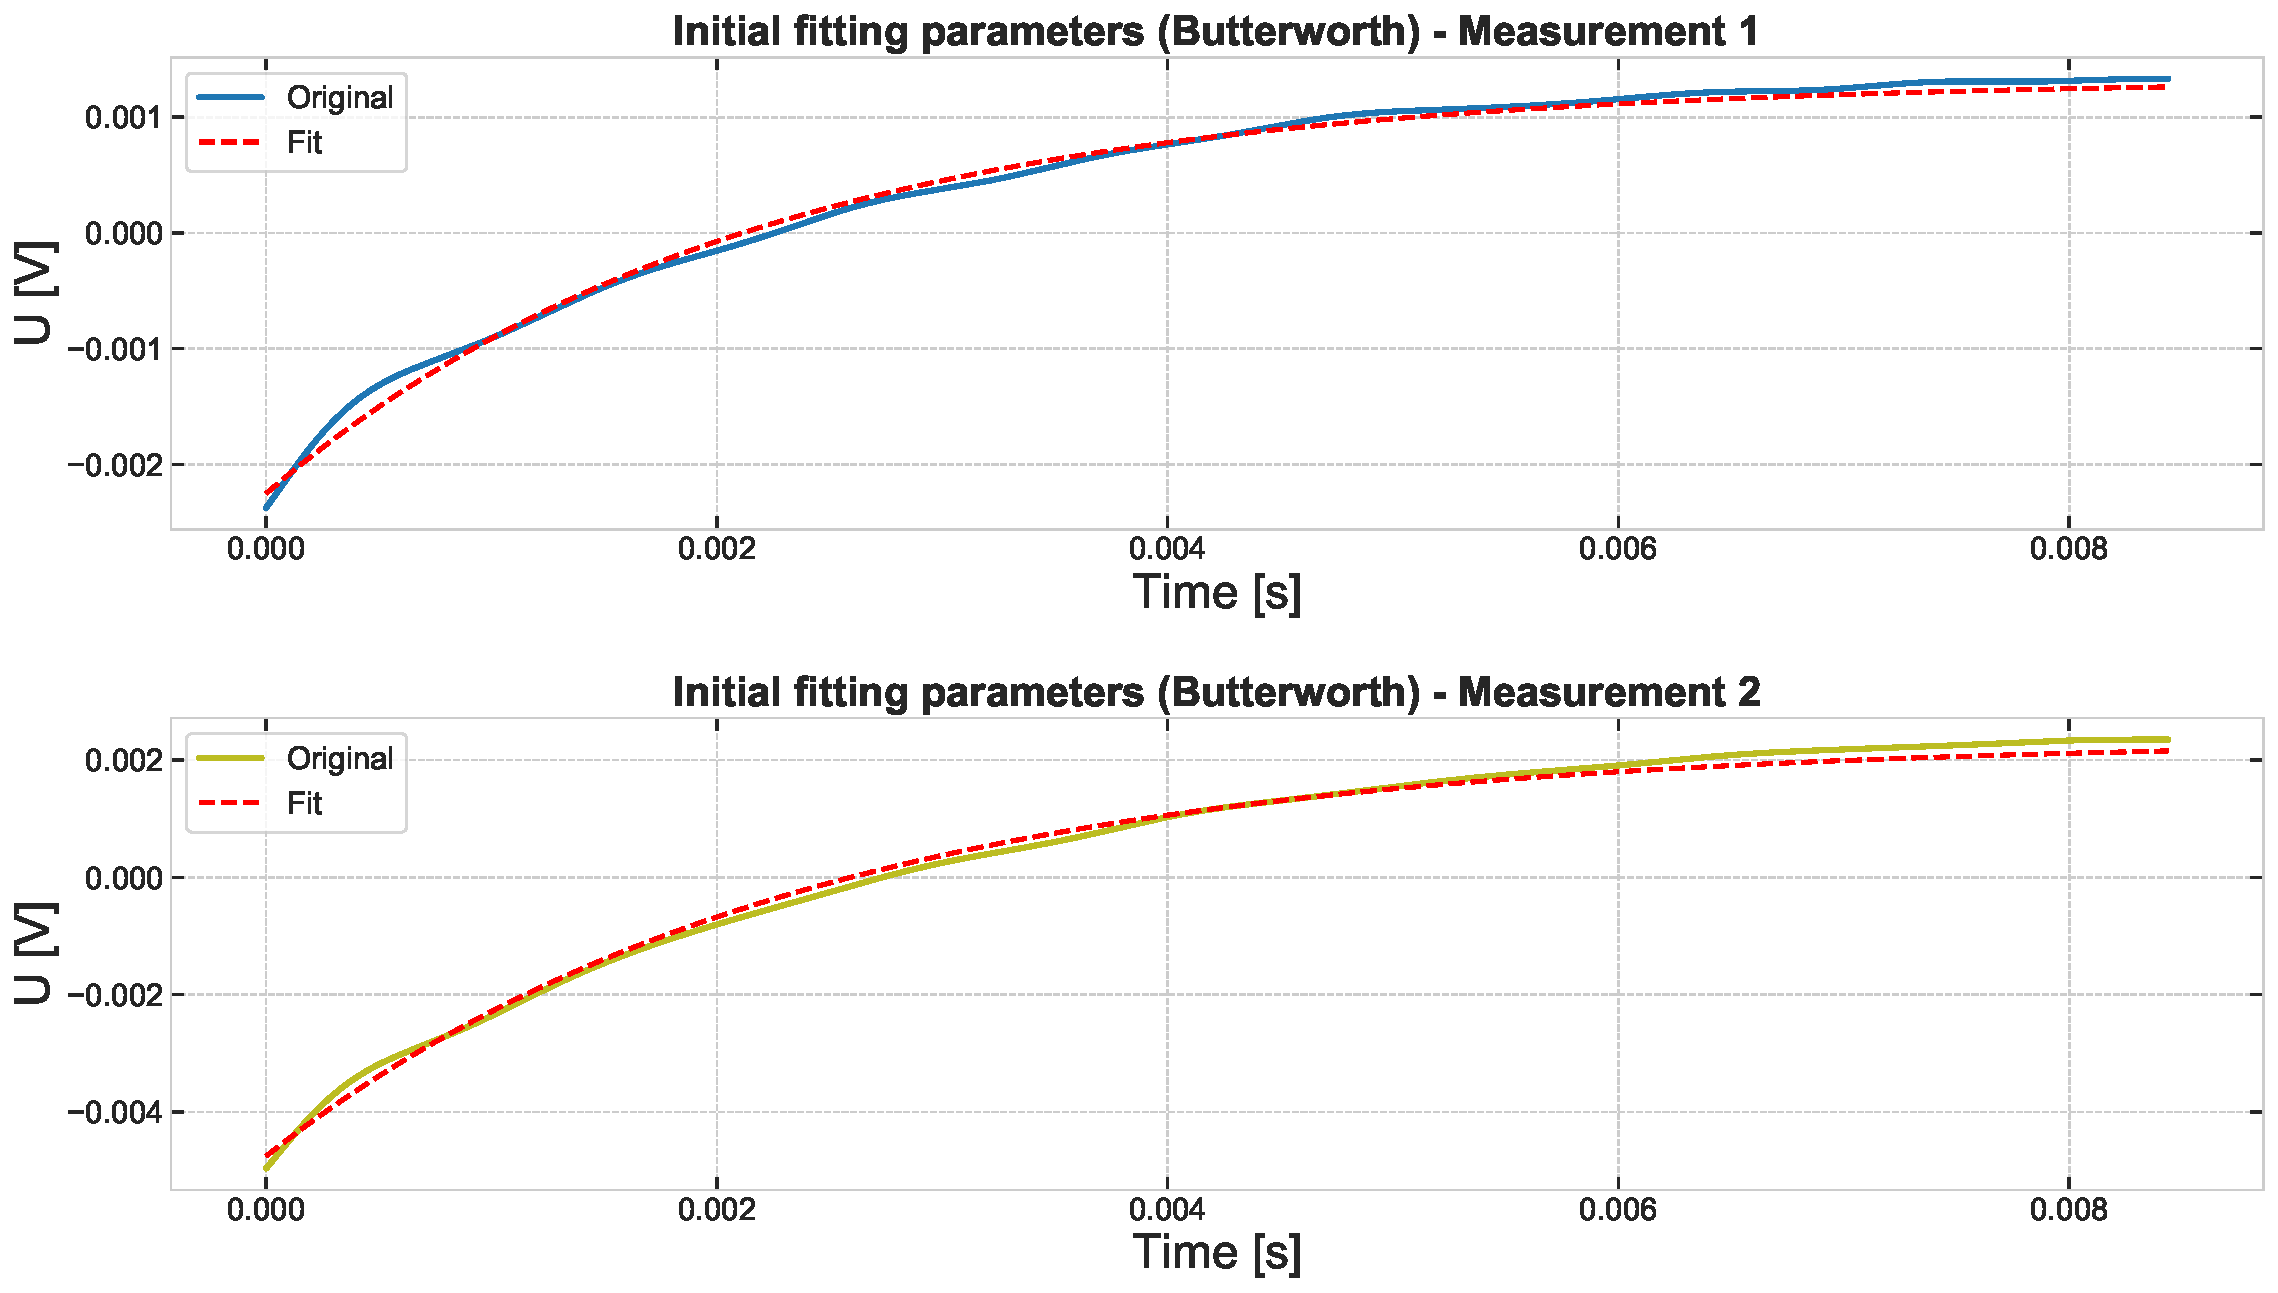
\includegraphics[width=\textwidth]{images/tau_butterworth_fitted_initial.pdf}
    \captionof{figure}{A $\tau$ mérése során kapott, aluláteresztő szűrőn átengedett jelalak egyik felfutó élére illesztett paraméteres görbe az első lépésben becsült együtthatóival ábrázolva.} \label{fig:9}
\end{center}
\begin{center}
    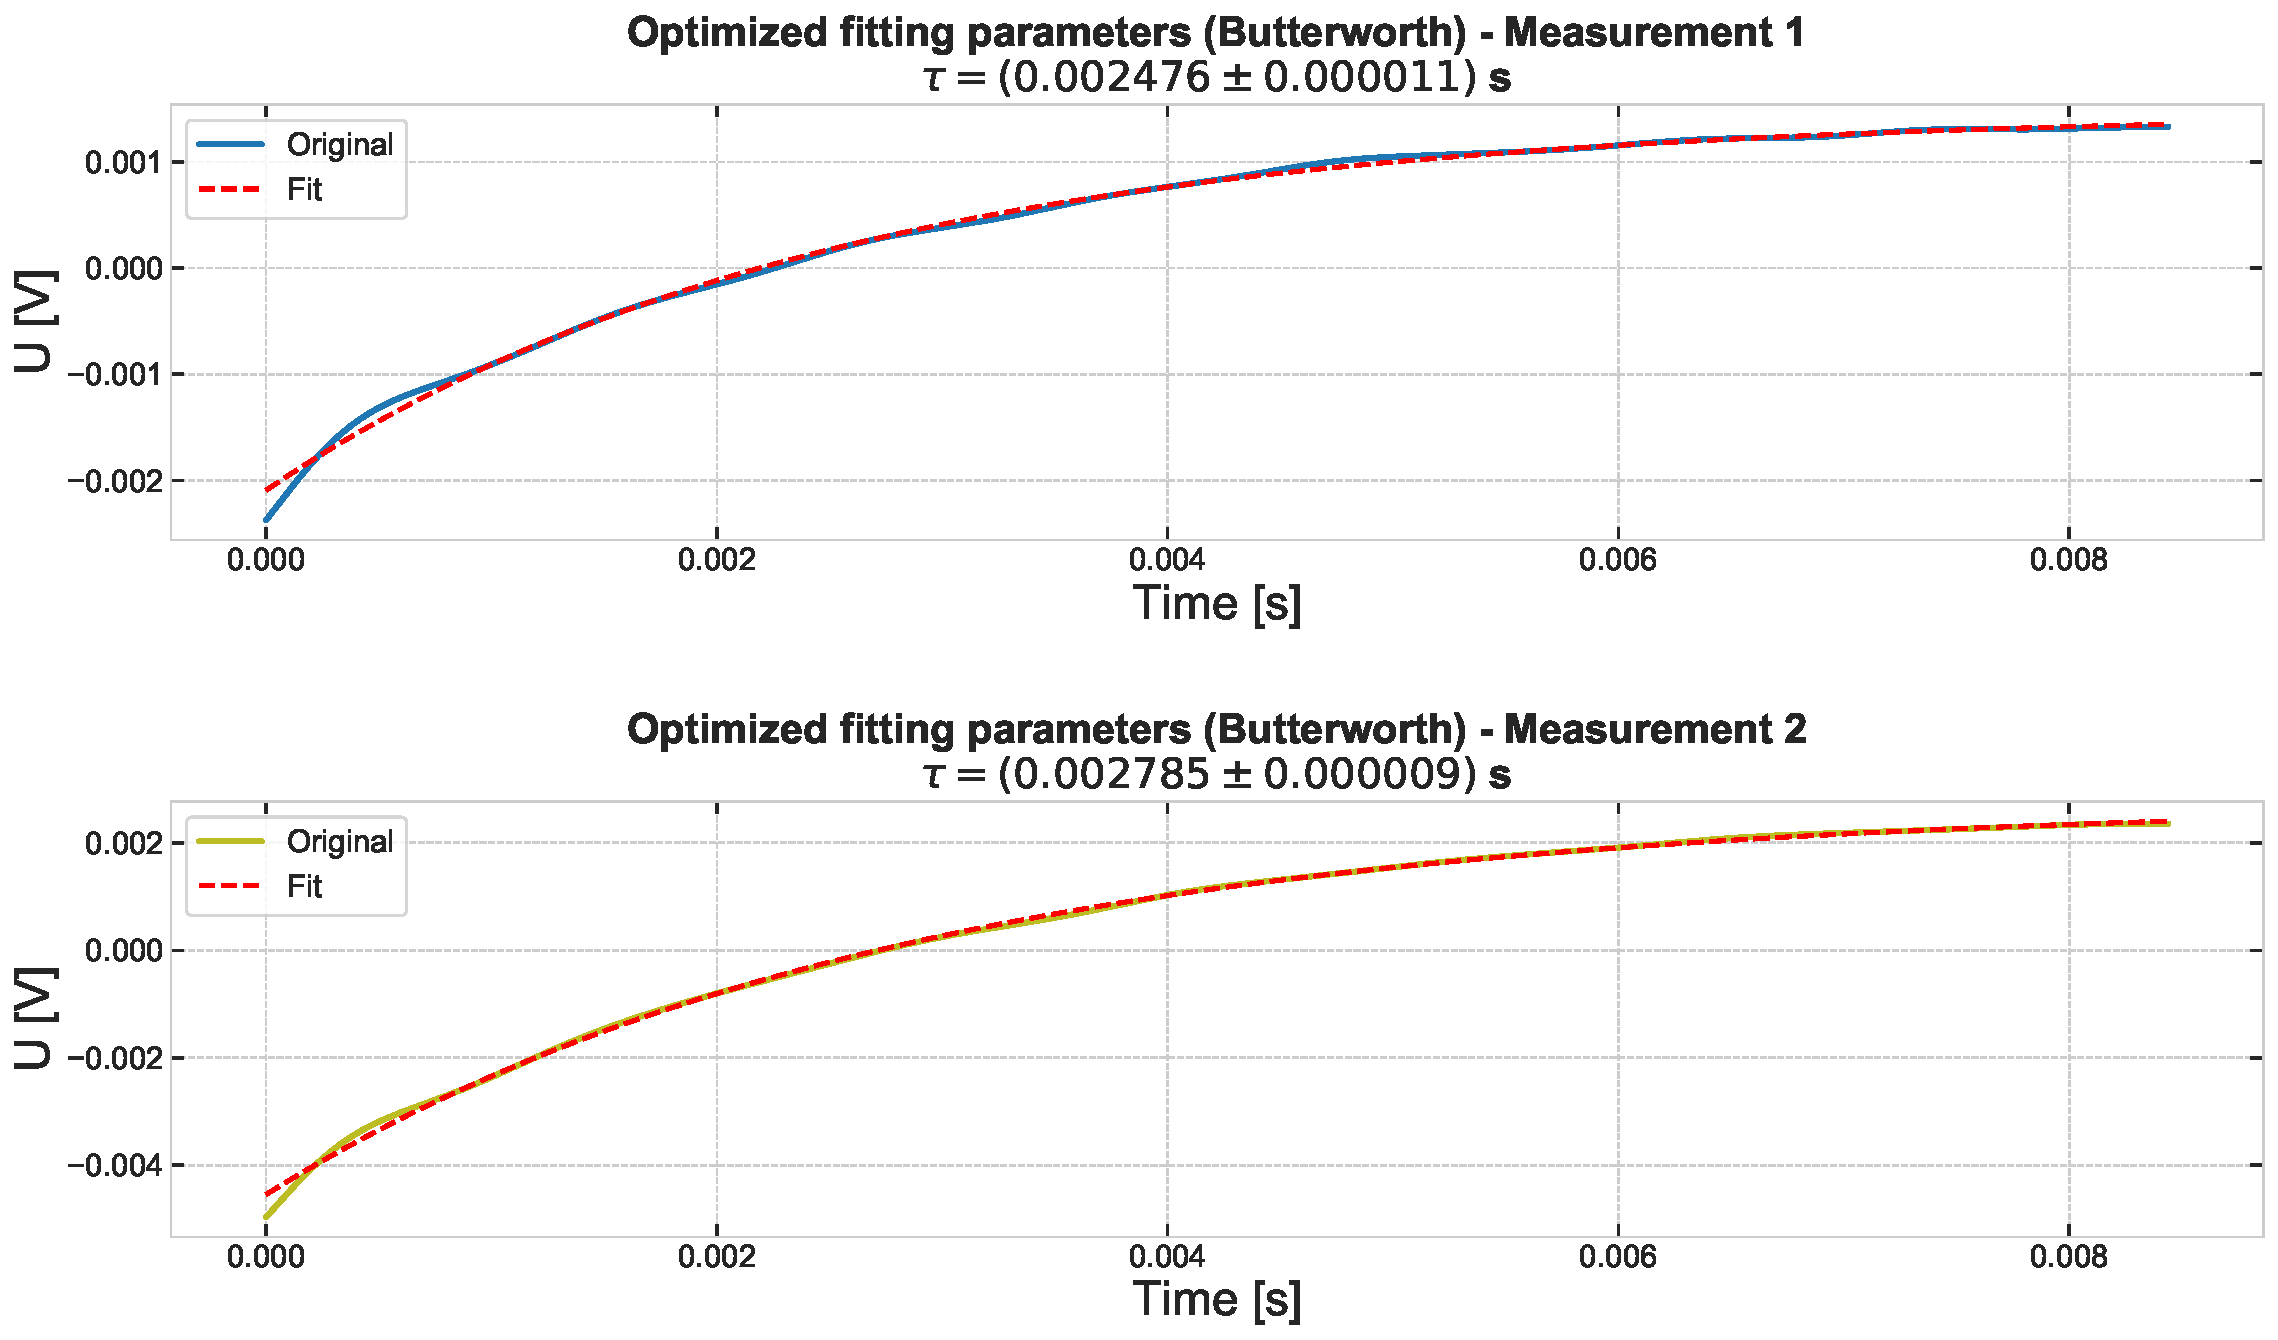
\includegraphics[width=\textwidth]{images/tau_butterworth_fitted_optimized.pdf}
    \captionof{figure}{A $\tau$ mérése során kapott, aluláteresztő szűrőn átengedett jelalak egyik felfutó élére illesztett paraméteres görbe a függvényillesztési iterációk után optimalizált együtthatóival ábrázolva.} \label{fig:10}
\end{center}
\vspace*{\fill}
\newpage
\topskip0pt
\vspace*{\fill}
\begin{center}
    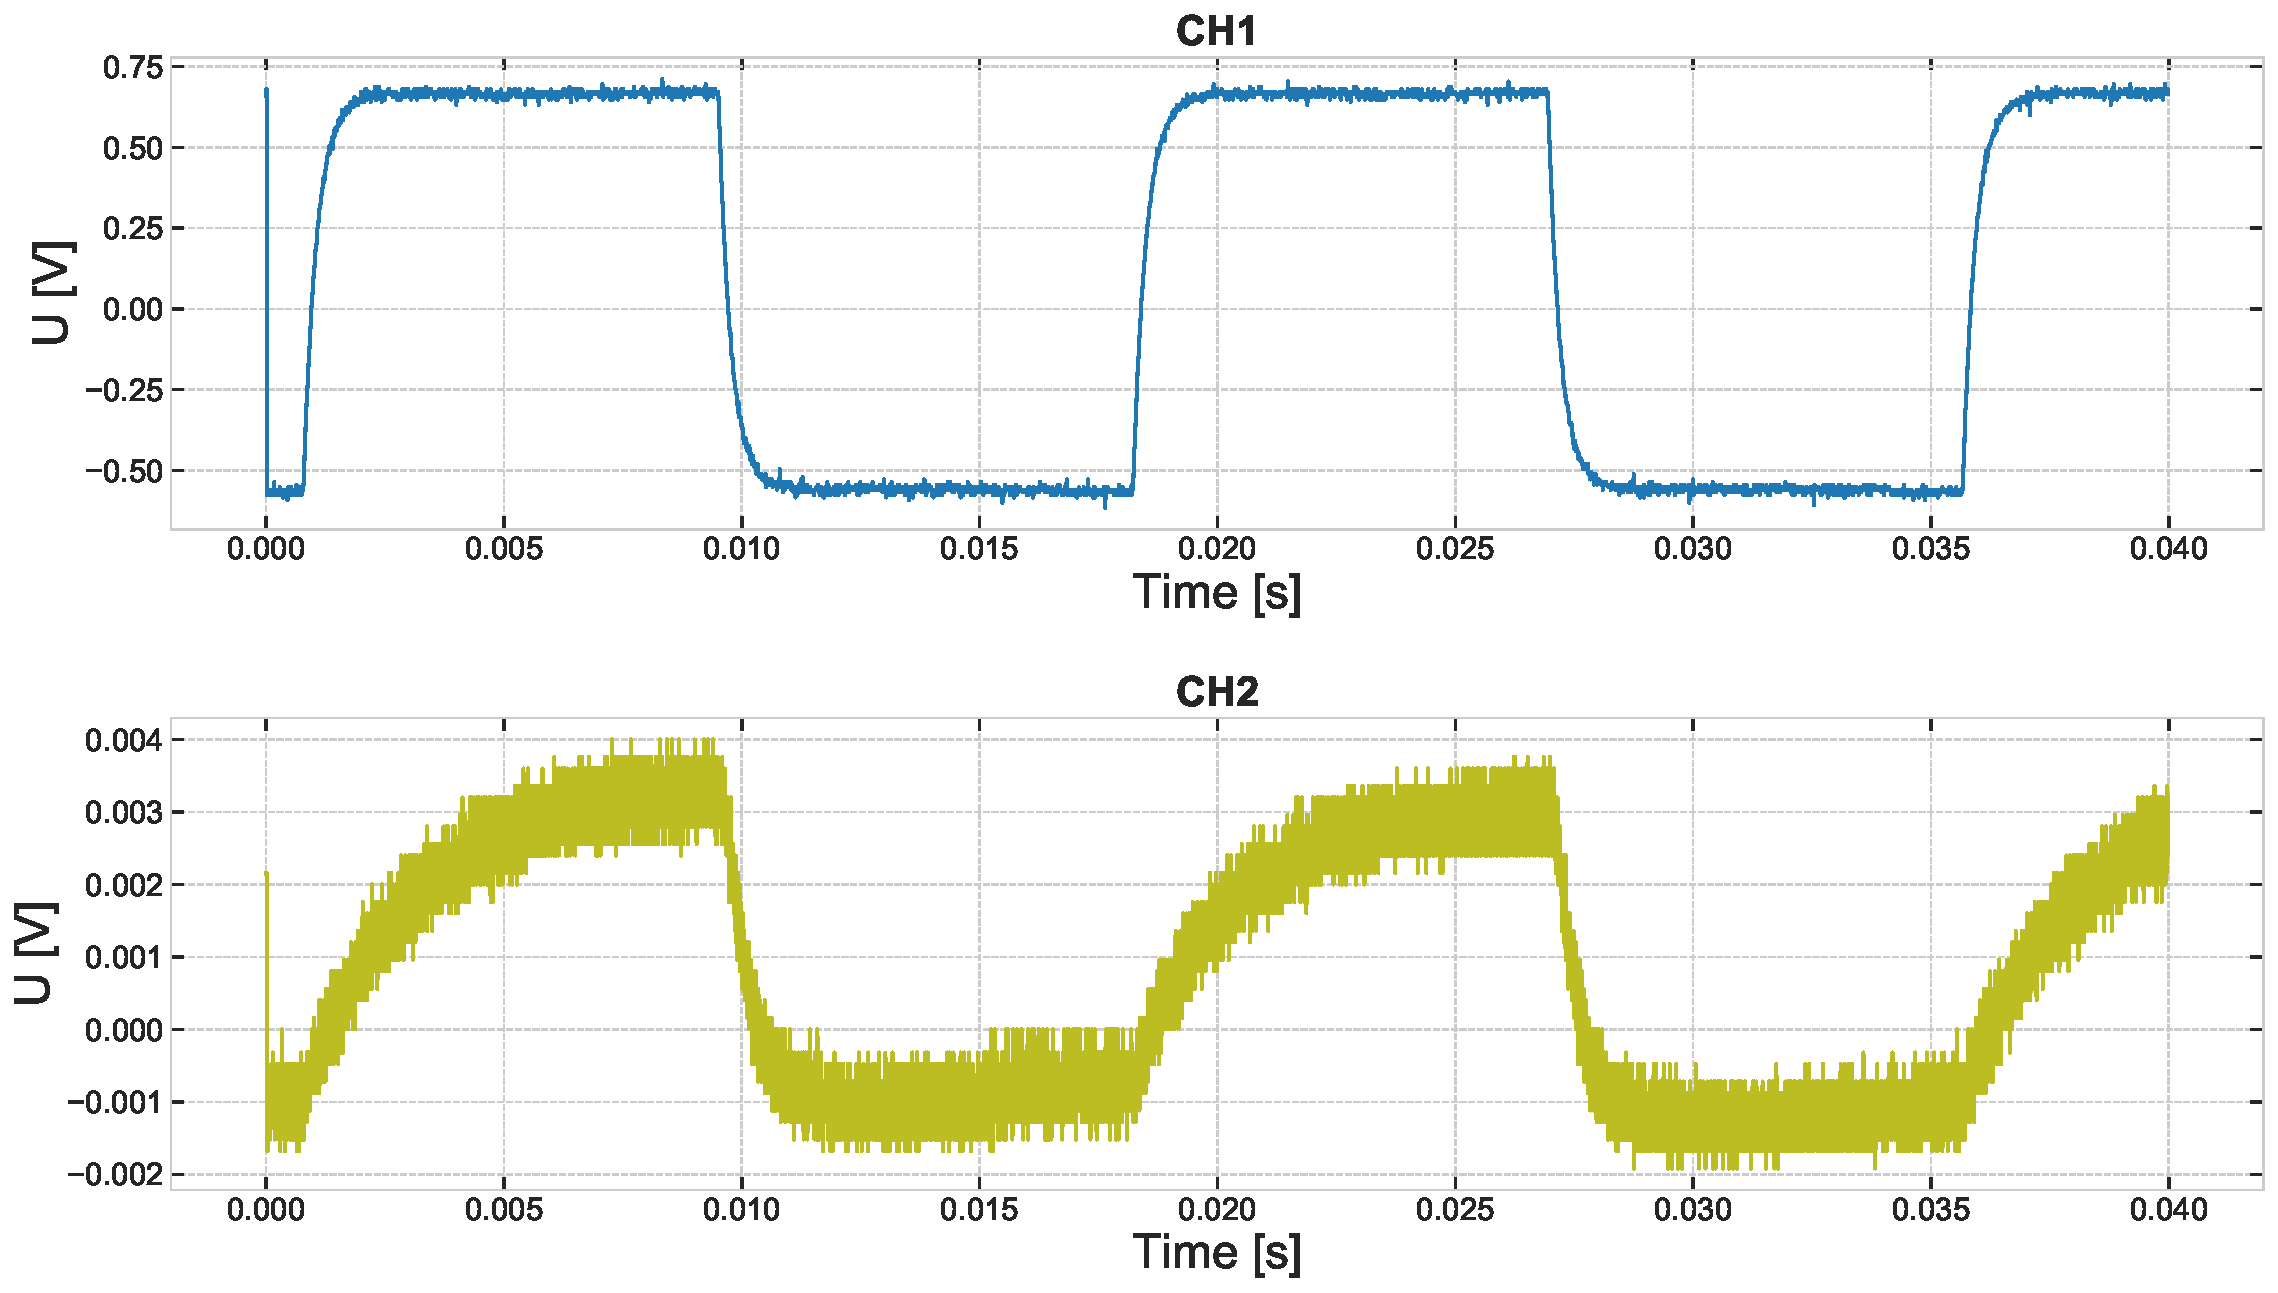
\includegraphics[width=\textwidth]{images/mag_channels.pdf}
    \captionof{figure}{A $T_{2}$ időállandót kimérendő, a Föld mágneses terét ellensúlyozó és így a minta helyén a mágneses teret teljesen kioltó áramot kapcsoltunk a Helmoltz-tekercsekre. A tekercsre kapcsolt jelalak a felső, míg a fotódióda jele az alsó ábrán látható.} \label{fig:11}
\end{center}
\begin{center}
    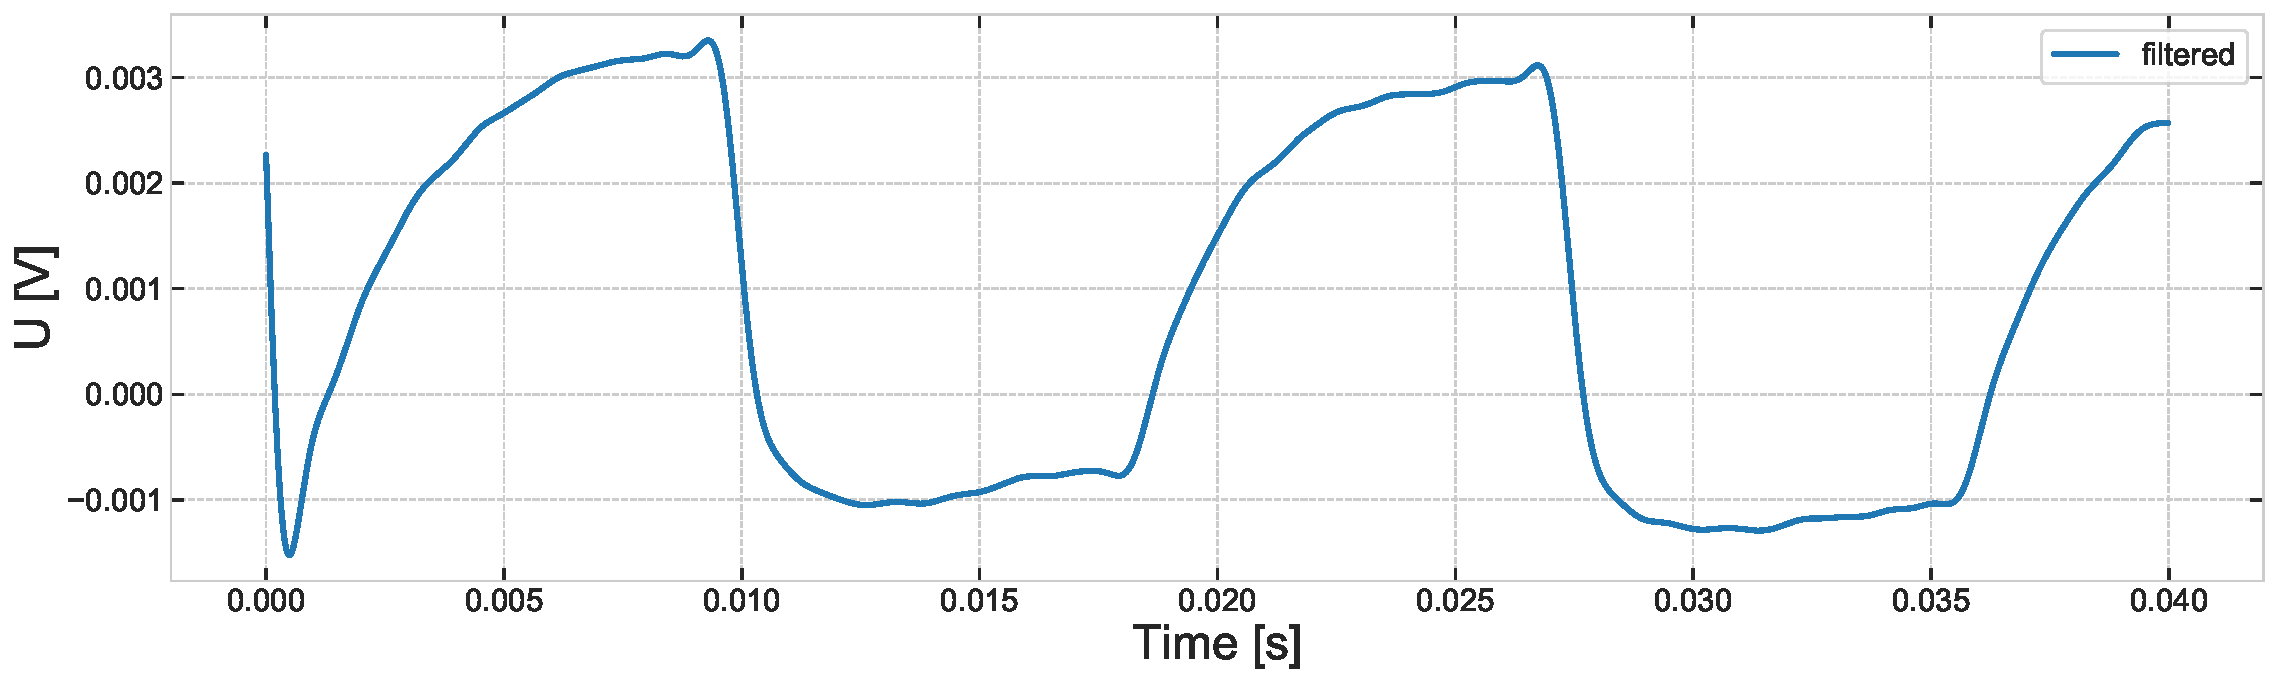
\includegraphics[width=\textwidth]{images/mag_butterworth.pdf}
    \captionof{figure}{A fotodióda jele egy $f_{C} = 1000$ Hz levágási frekvenciával rendelkező aluláteresztő szűrőn átengedve.} \label{fig:12}
\end{center}
\begin{center}
    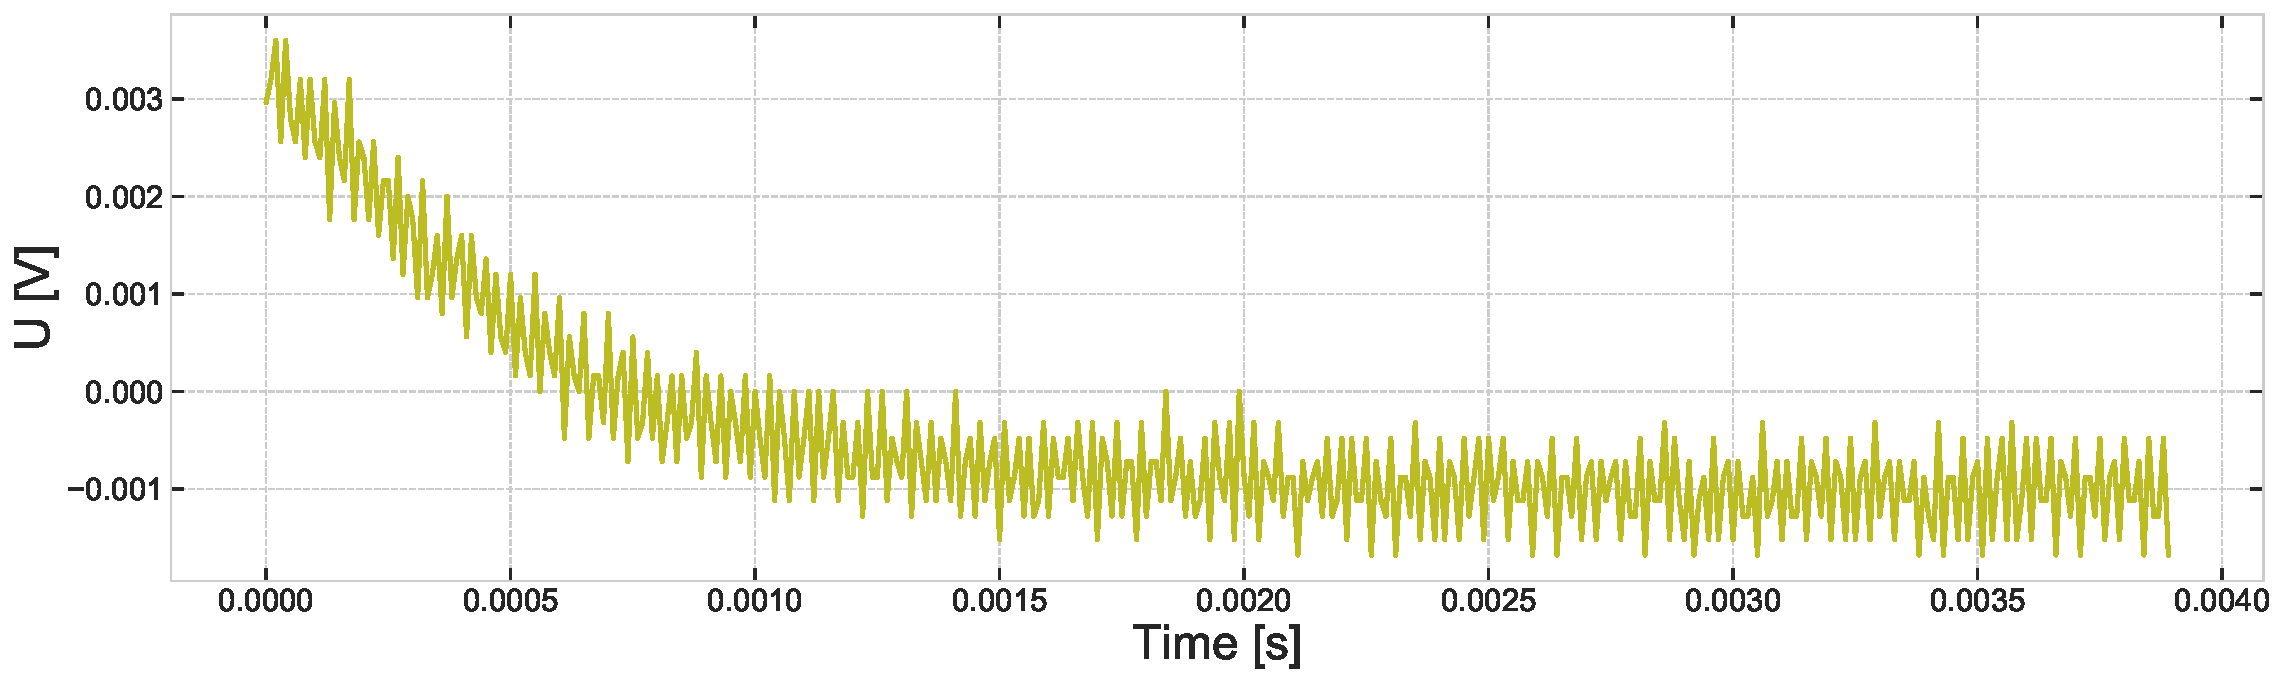
\includegraphics[width=\textwidth]{images/mag_sliced.pdf}
    \captionof{figure}{A $T_{2}$ mérése során kapott jelalak egyik periódusának lefutó éle. A jel kezdőpontja a $t=0$-ba van eltolva.} \label{fig:13}
\end{center}
\begin{center}
    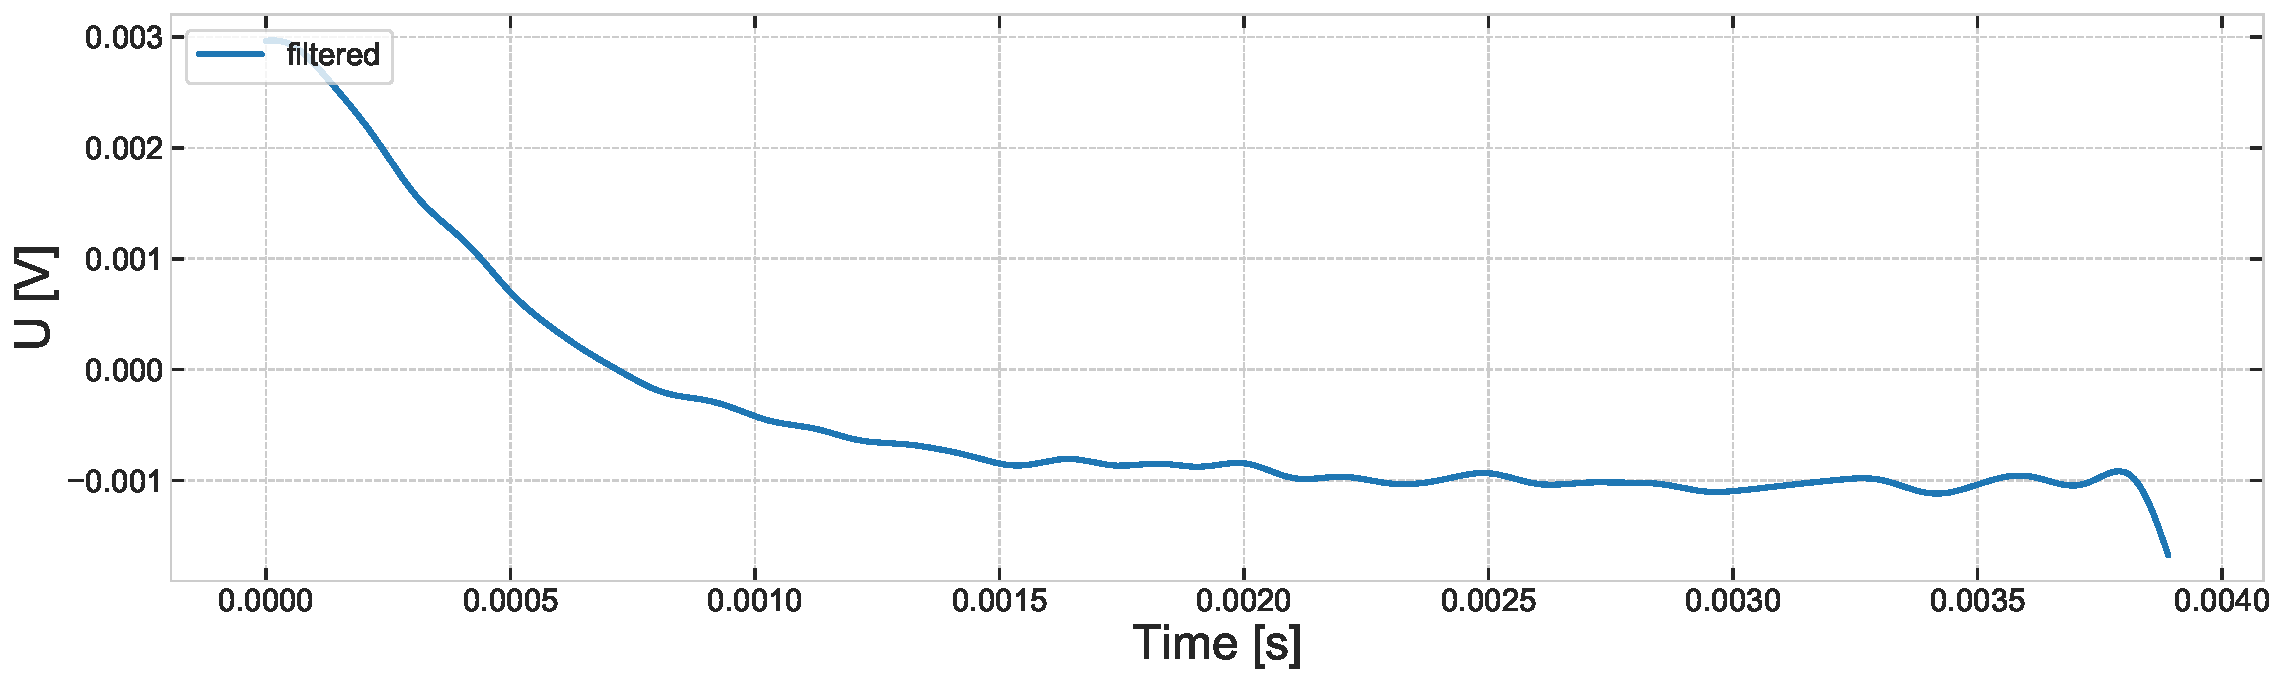
\includegraphics[width=\textwidth]{images/mag_sliced_butterworth.pdf}
    \captionof{figure}{A $T_{2}$ mérése során kapott jelalak egyik periódusának lefutó éle, egy $f_{C} = 1000$ Hz levágási frekvenciával rendelkező aluláteresztő szűrőn átengedve. A jel kezdőpontja a $t=0$-ba van eltolva.} \label{fig:14}
\end{center}
\vspace*{\fill}
\newpage
\topskip0pt
\vspace*{\fill}
\begin{center}
    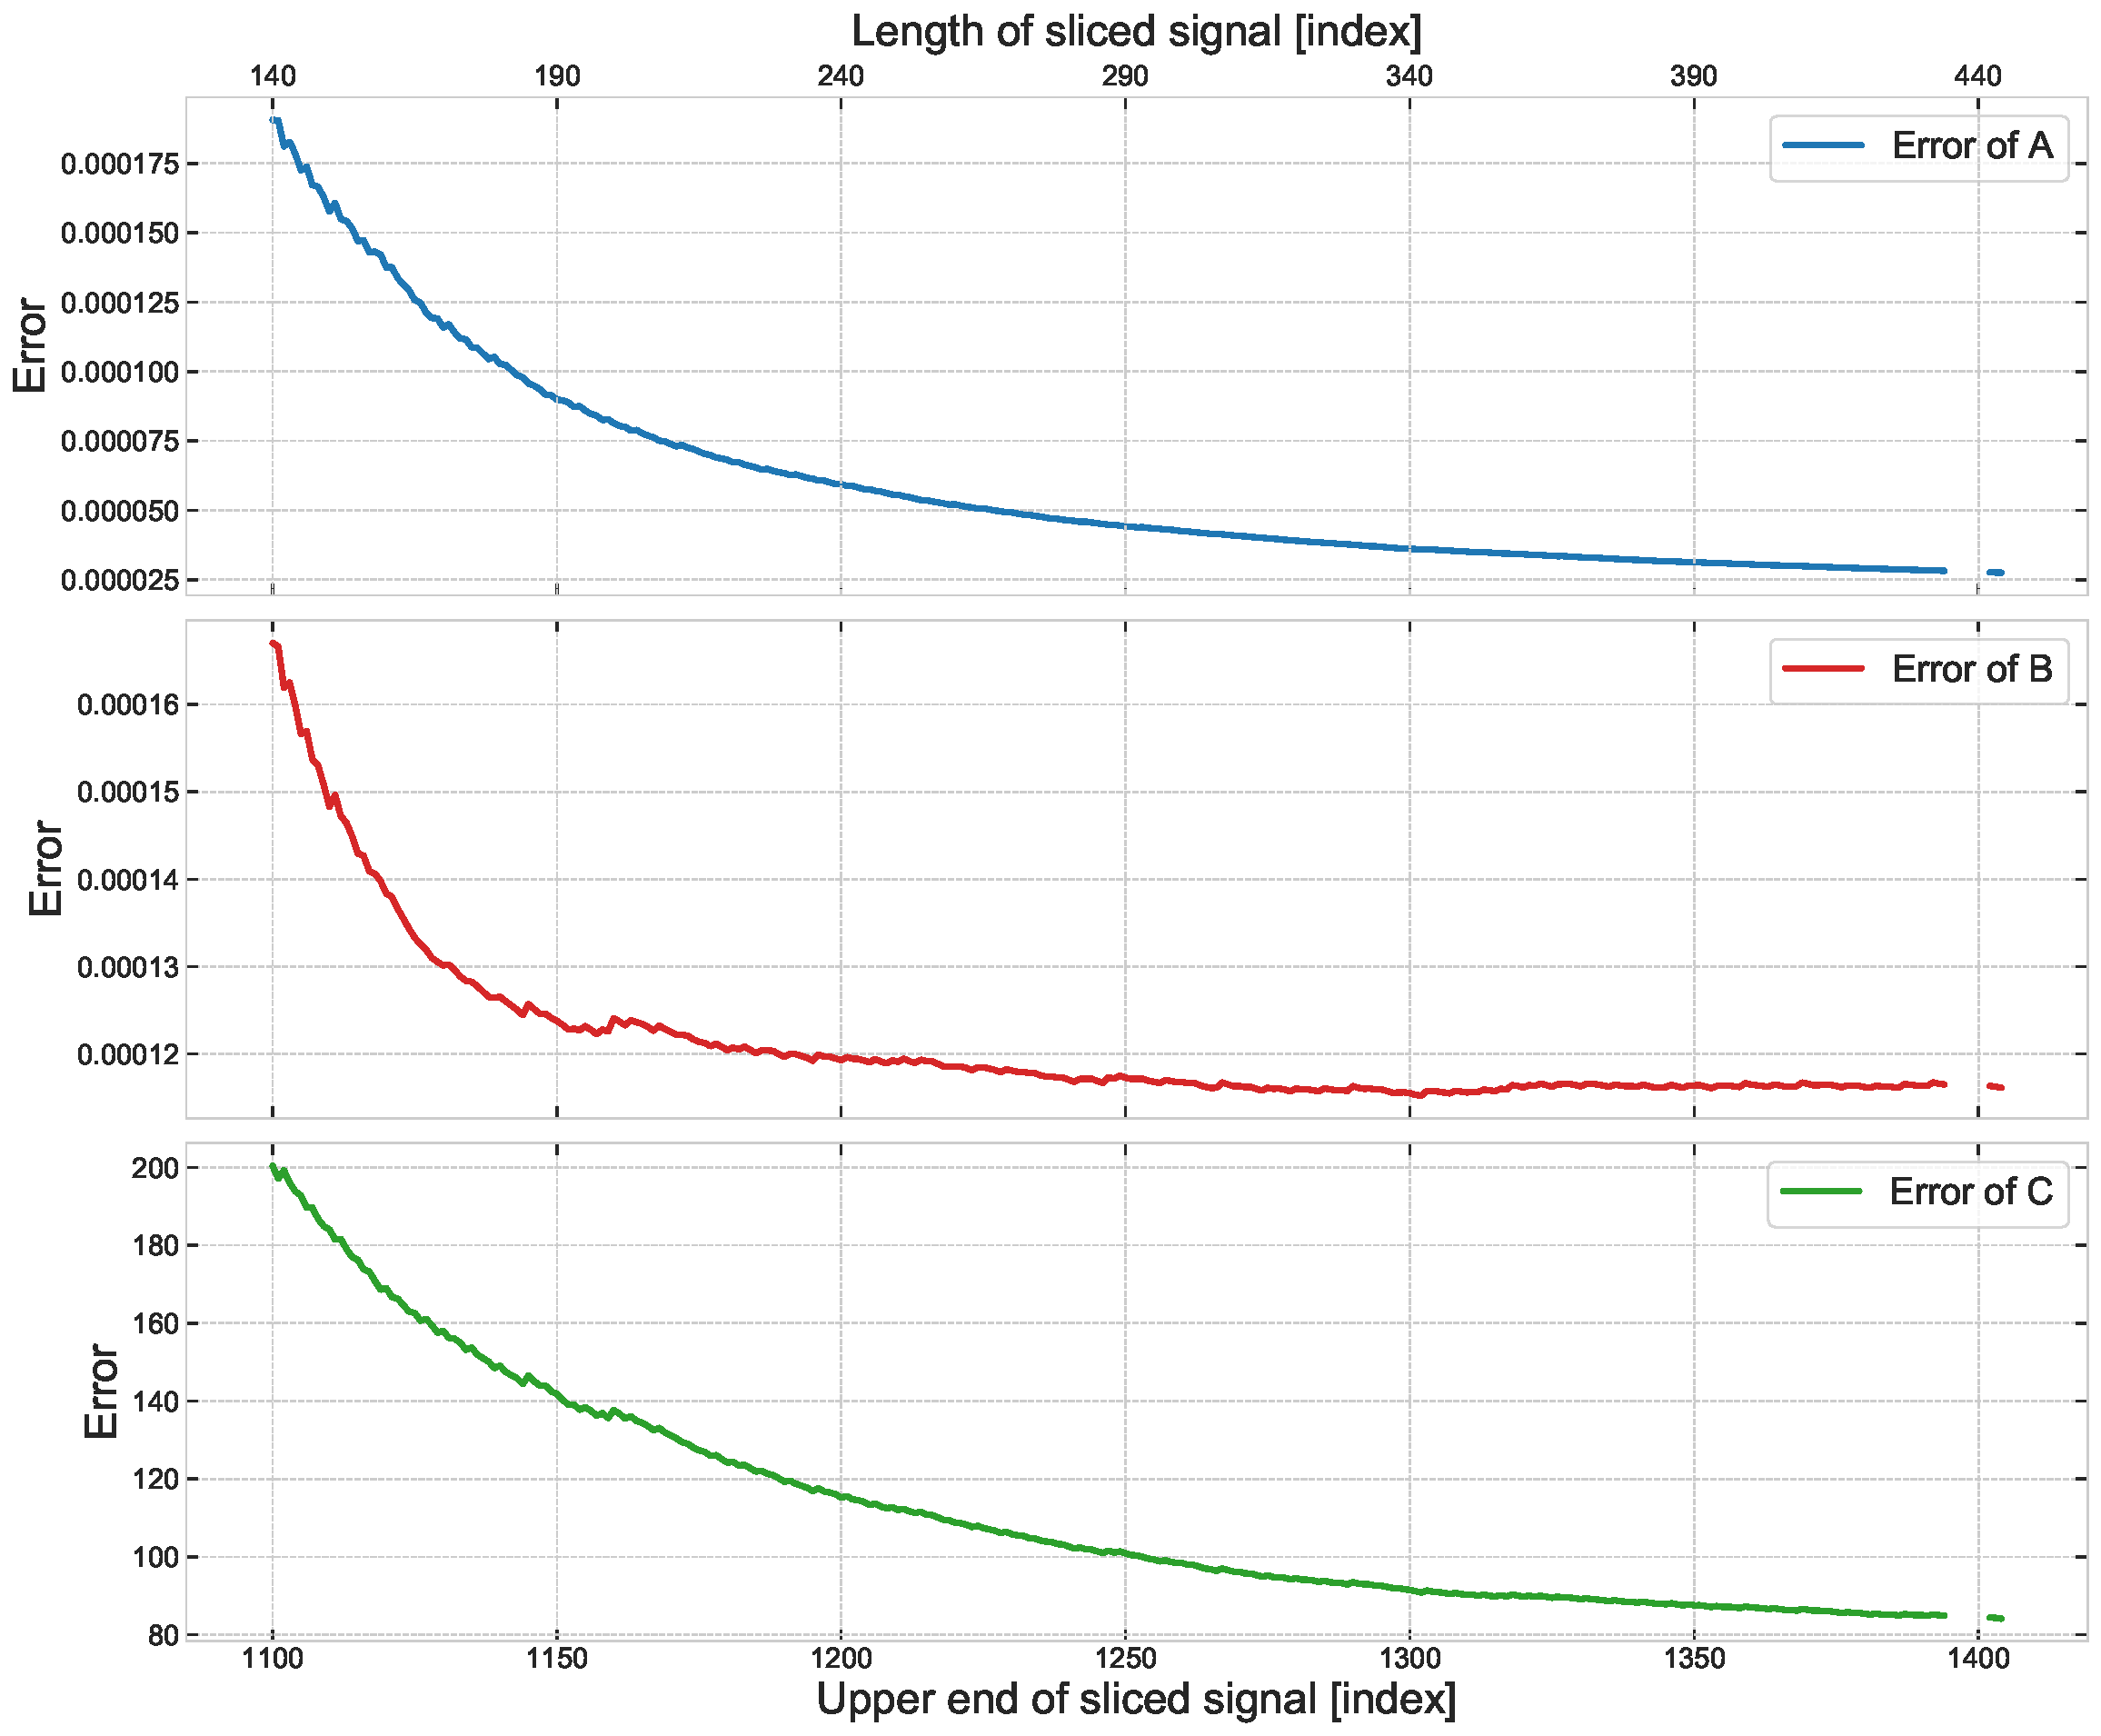
\includegraphics[width=\textwidth]{images/mag_fitted_errors.pdf}
    \captionof{figure}{A lefutó élek pontos hosszának kiválasztása az arra történő függvényillesztés standard hibájának elemzésével történt, mely után az elérhető legkisebb hibához tartozó pontnál választottam meg az él hosszát.} \label{fig:15}
\end{center}
\vspace*{\fill}
\newpage
\topskip0pt
\vspace*{\fill}
\begin{center}
    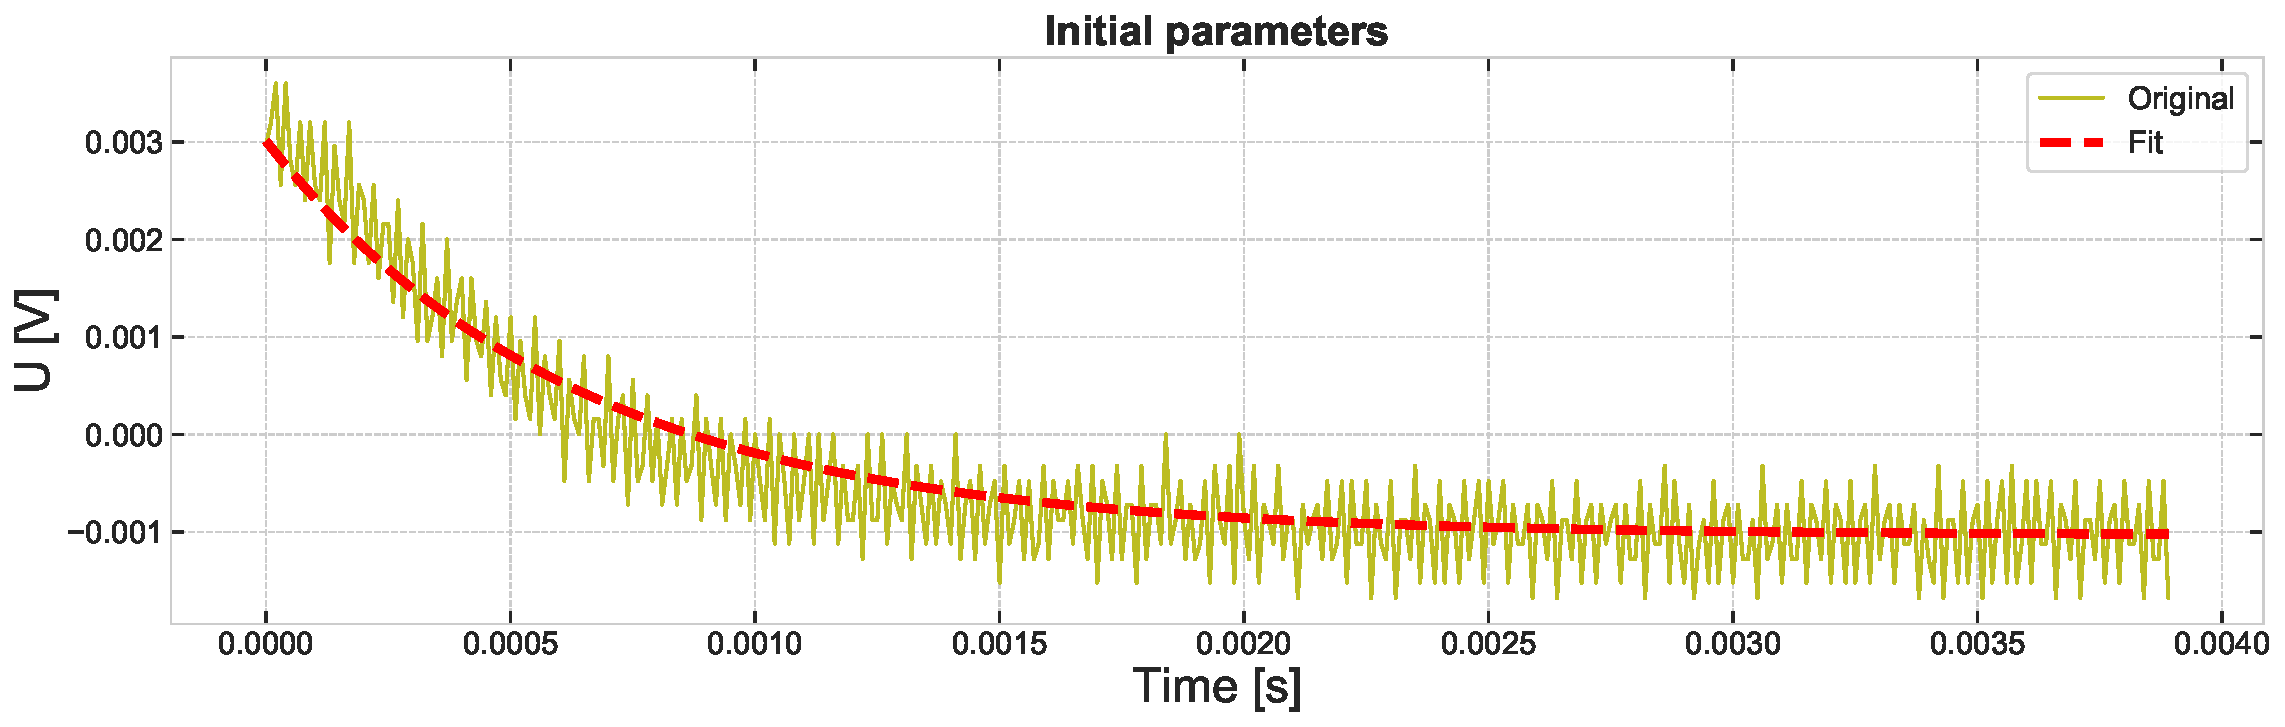
\includegraphics[width=\textwidth]{images/mag_fitted_initial.pdf}
    \captionof{figure}{A $T_{2}$ mérése során kapott, szűrés nélküli jelalak egyik lefutó élére illesztett paraméteres görbe az első lépésben becsült együtthatóival ábrázolva.} \label{fig:16}
\end{center}
\begin{center}
    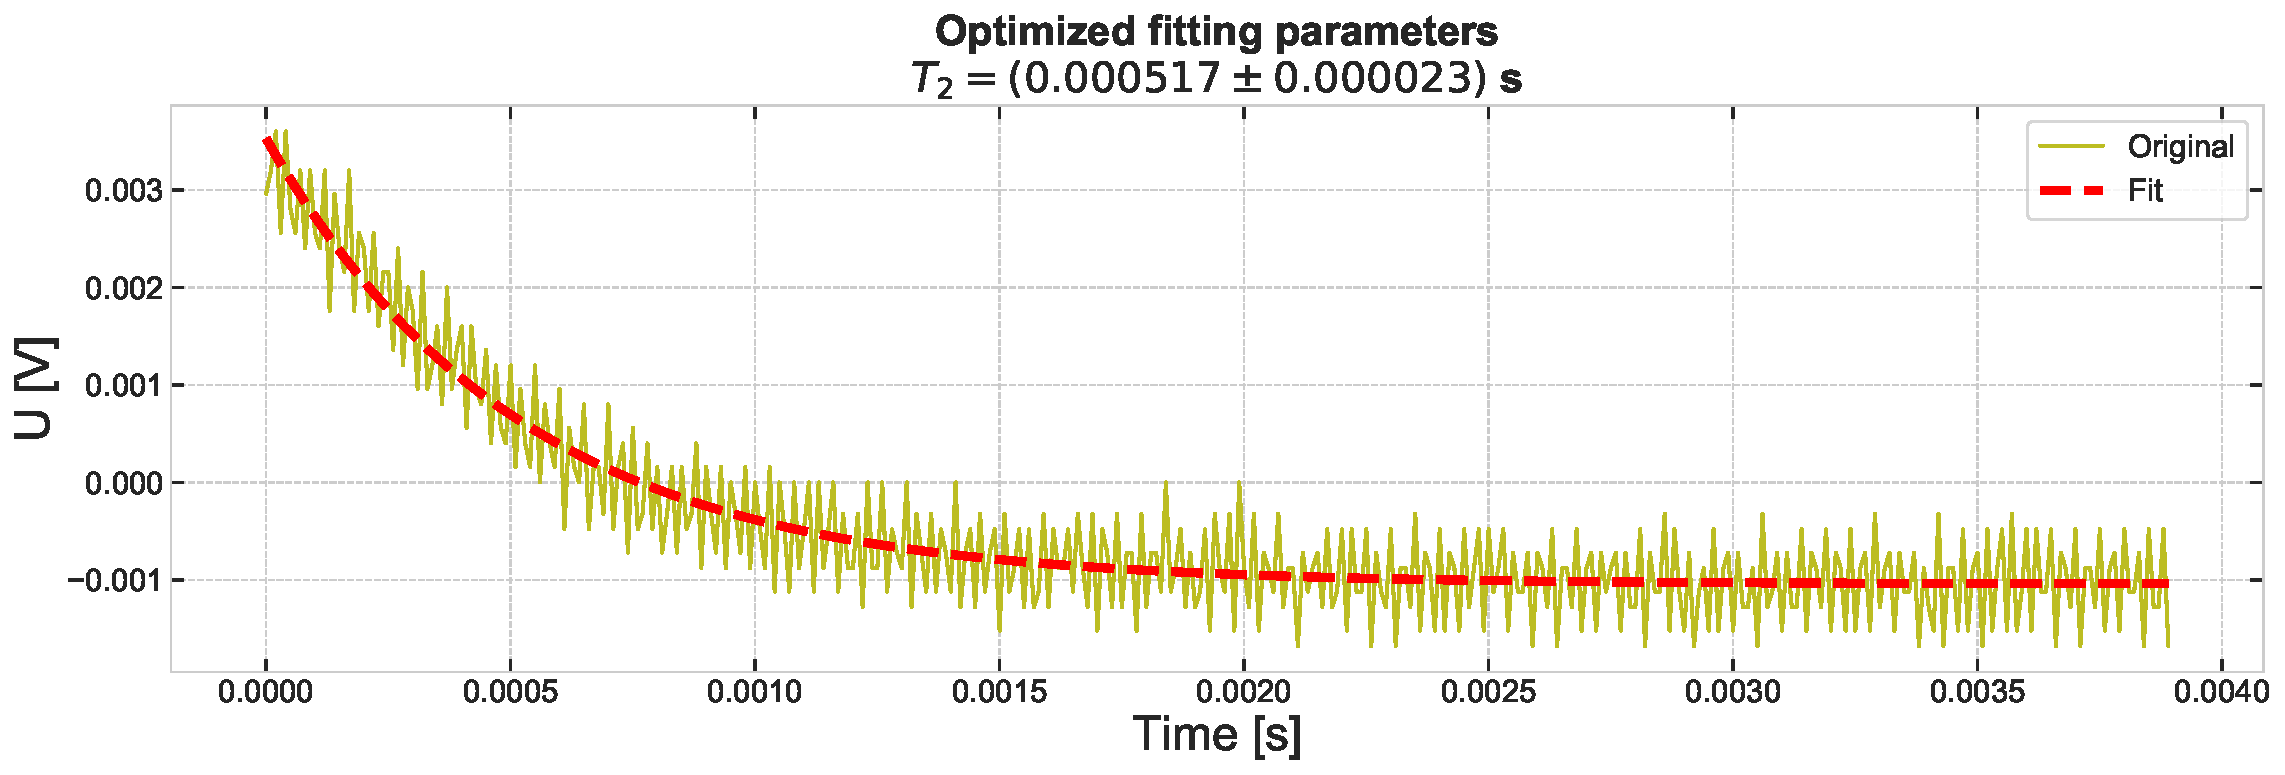
\includegraphics[width=\textwidth]{images/mag_fitted_optimized.pdf}
    \captionof{figure}{A $T_{2}$ mérése során kapott, szűrés nélküli jelalak egyik felfutó élére illesztett paraméteres görbe a függvényillesztési iterációk után optimalizált együtthatóival ábrázolva.} \label{fig:17}
\end{center}
\begin{center}
    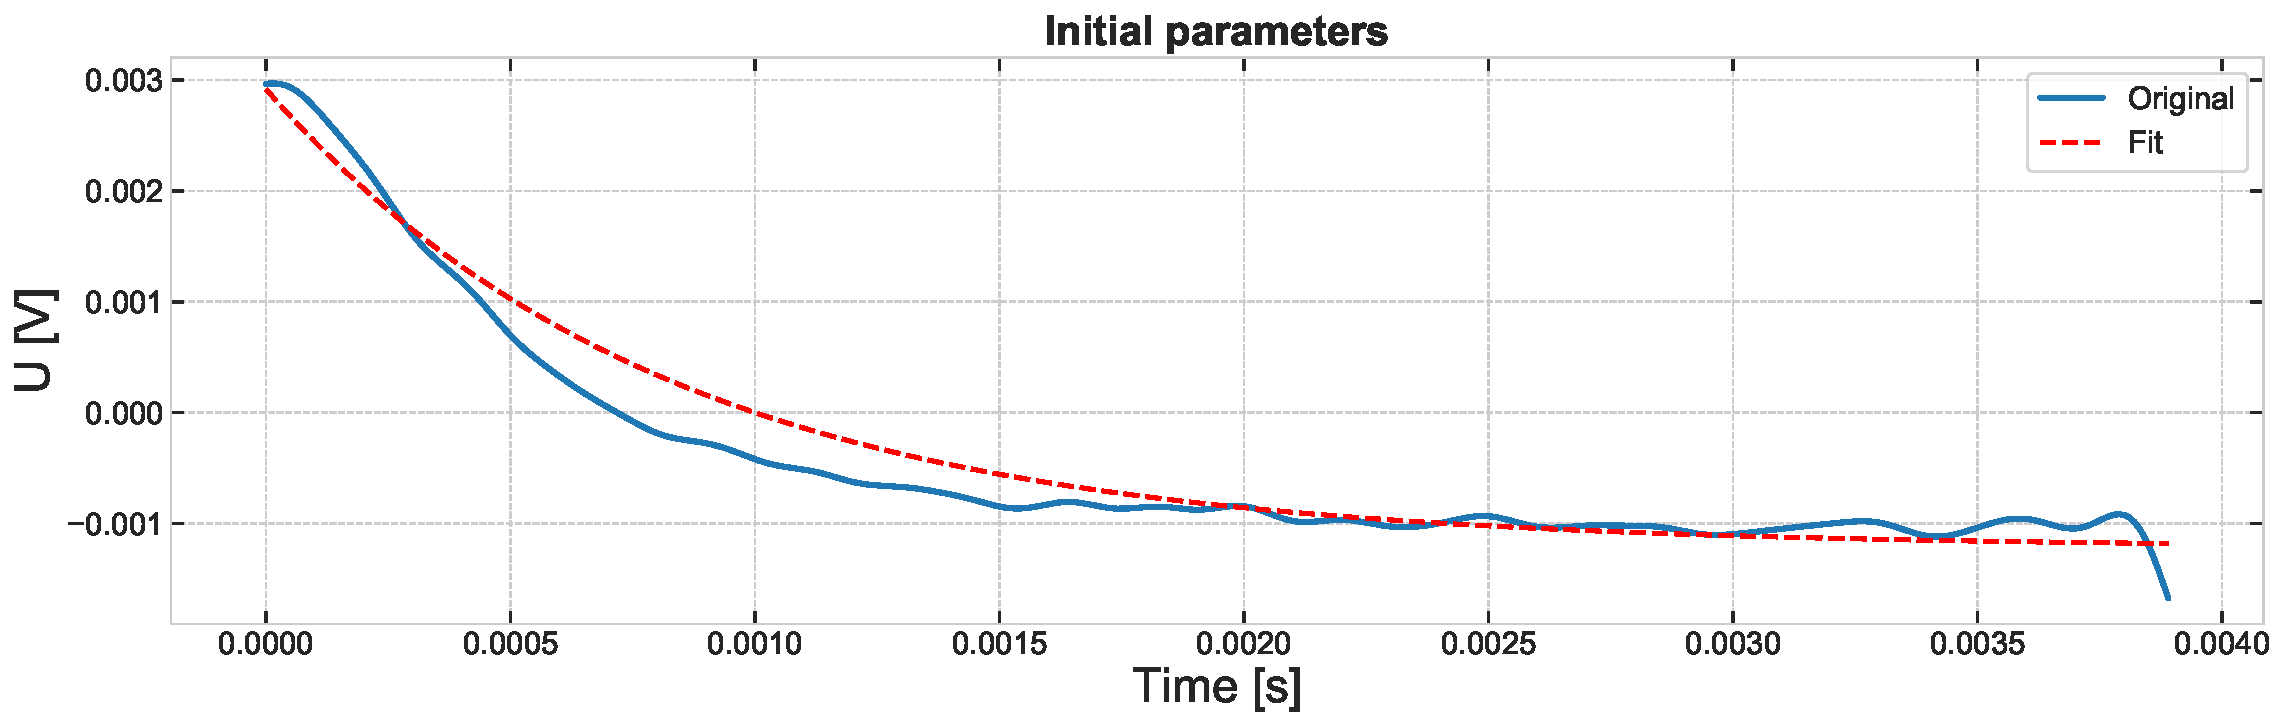
\includegraphics[width=\textwidth]{images/mag_butterworth_fitted_initial.pdf}
    \captionof{figure}{A $T_{2}$ mérése során kapott, aluláteresztő szűrőn átengedett jelalak egyik felfutó élére illesztett paraméteres görbe az első lépésben becsült együtthatóival ábrázolva.} \label{fig:18}
\end{center}
\begin{center}
    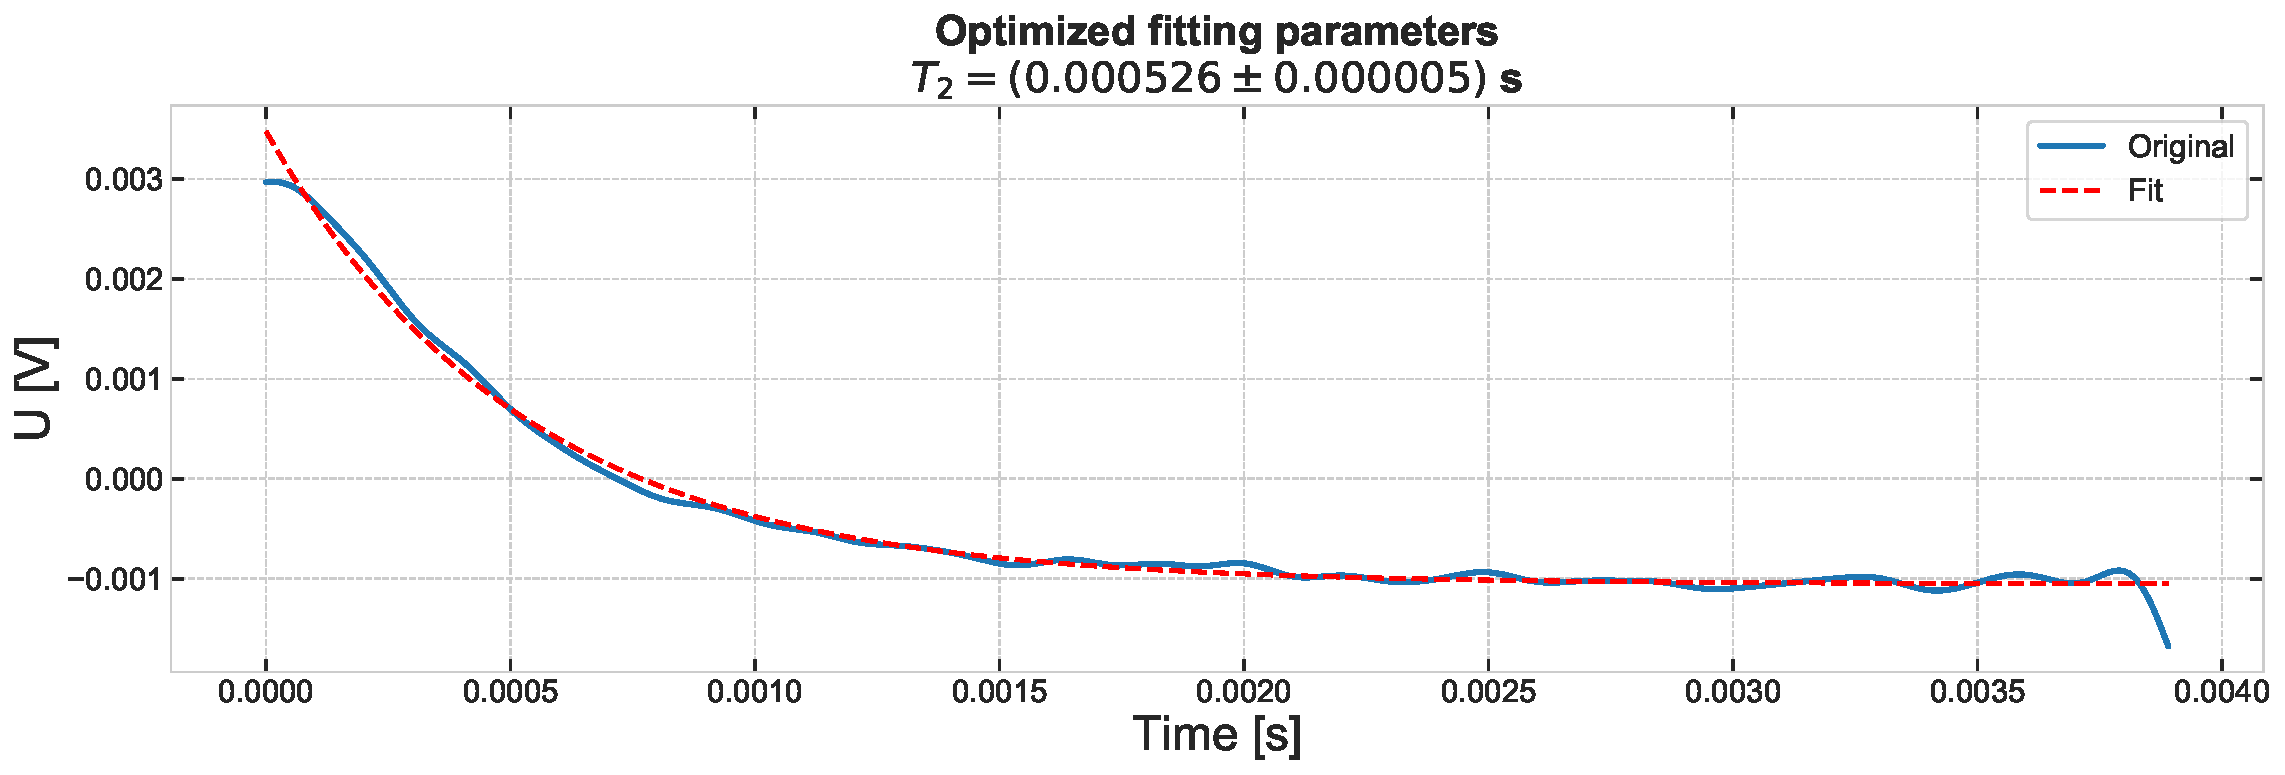
\includegraphics[width=\textwidth]{images/mag_butterworth_fitted_optimized.pdf}
    \captionof{figure}{A $T_{2}$ mérése során kapott, aluláteresztő szűrőn átengedett jelalak egyik felfutó élére illesztett paraméteres görbe a függvényillesztési iterációk után optimalizált együtthatóival ábrázolva.} \label{fig:19}
\end{center}
\vspace*{\fill}
\newpage
\topskip0pt
\vspace*{\fill}
\begin{center}
    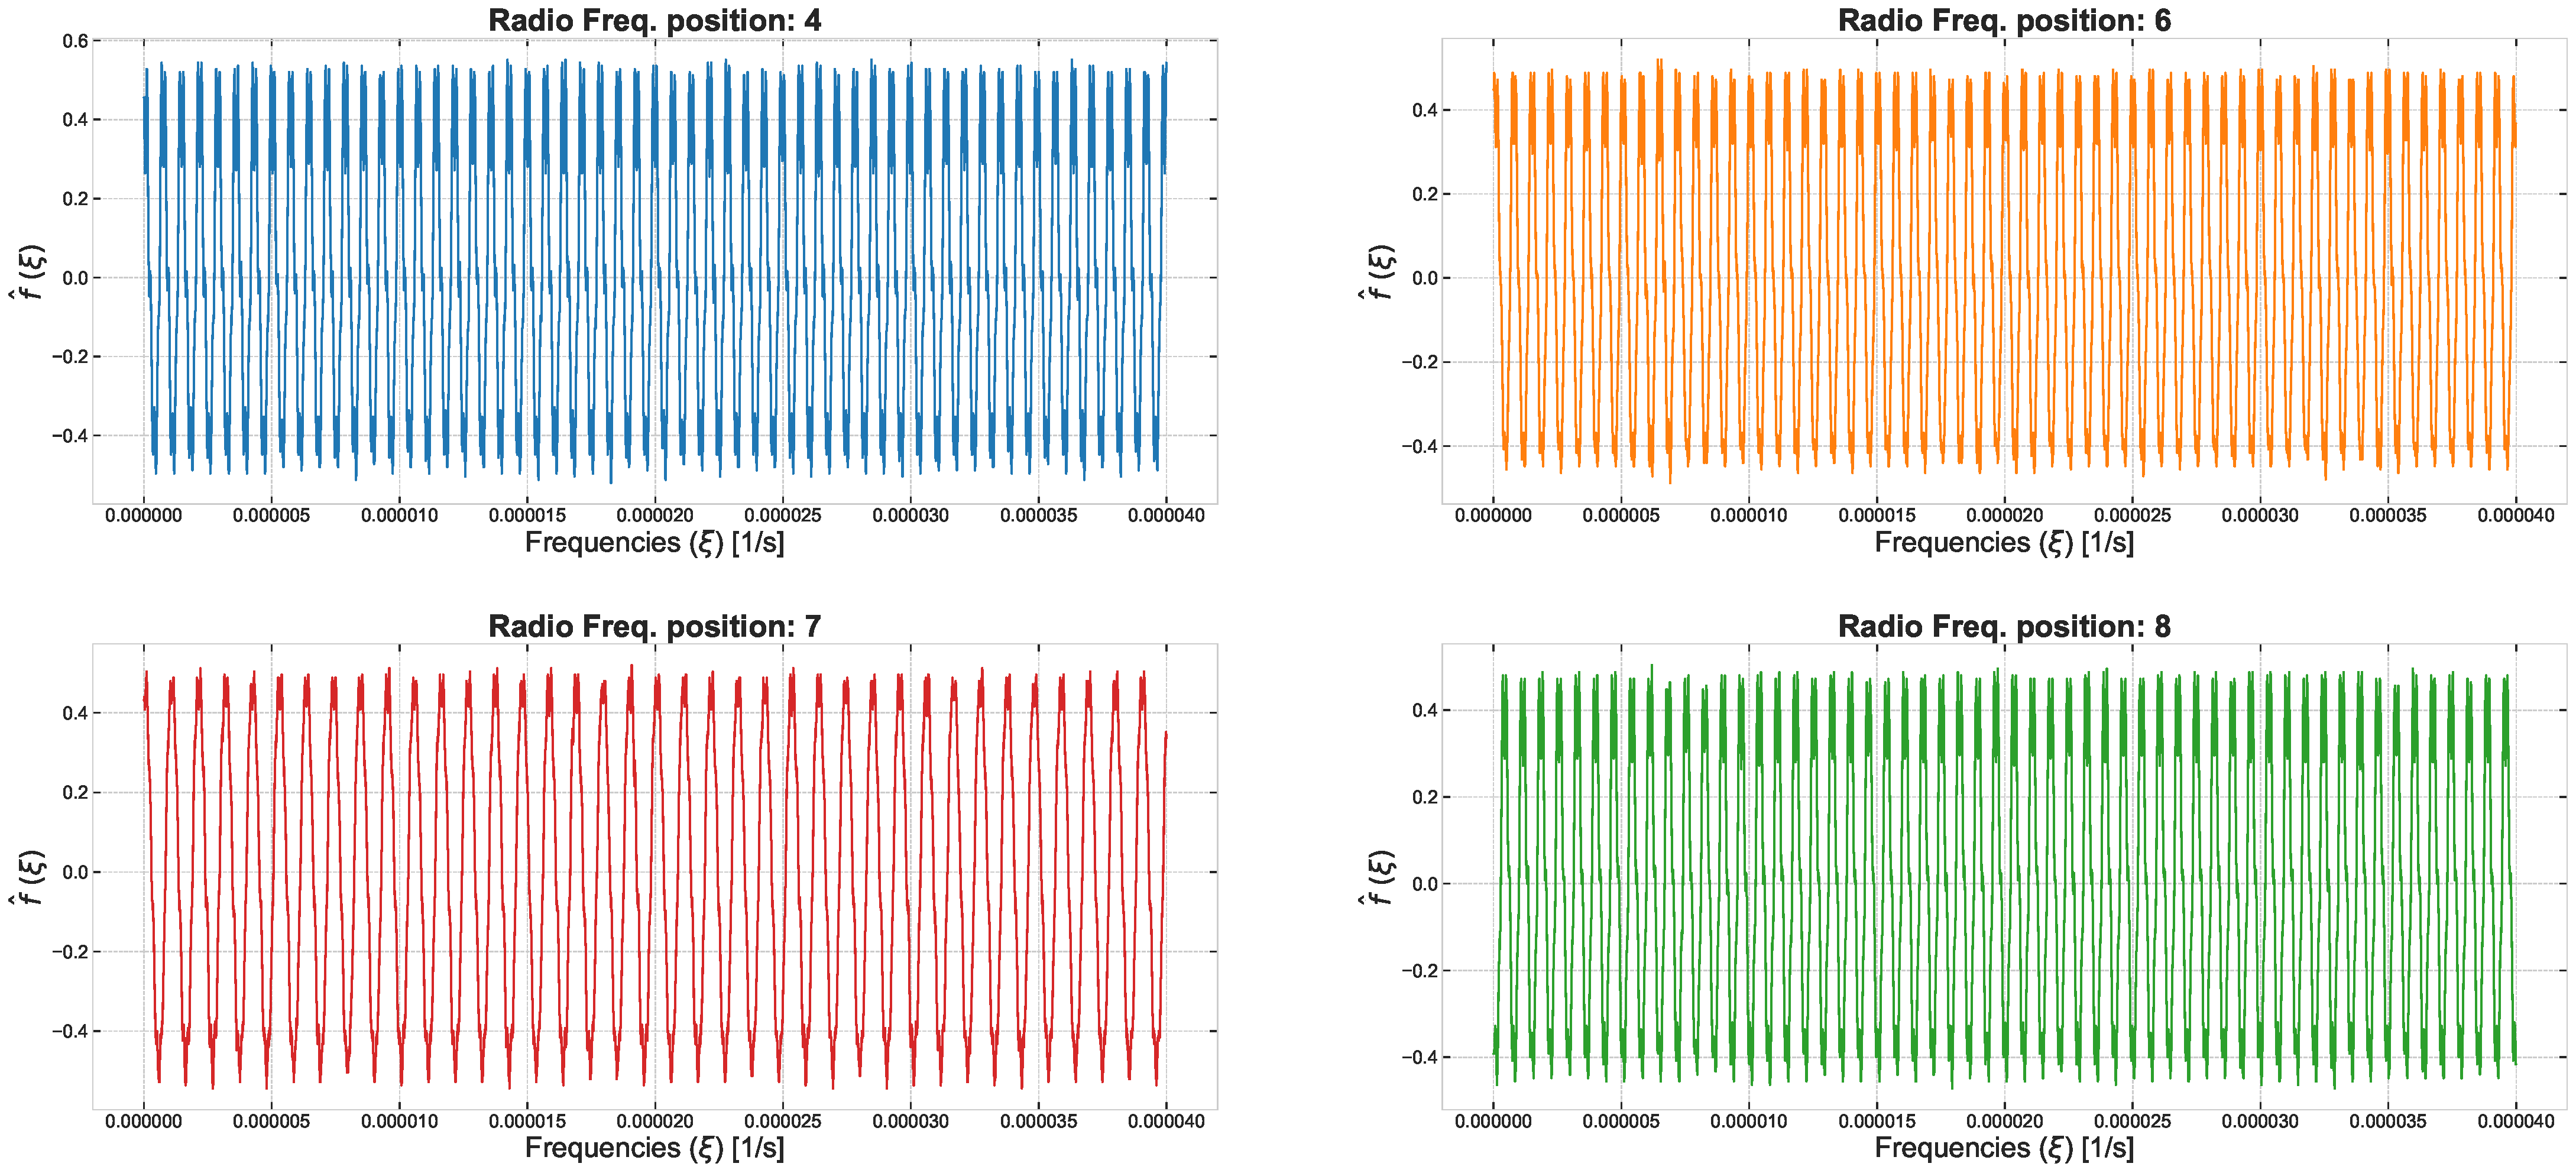
\includegraphics[width=\textwidth]{images/mag_freqs.pdf}
    \captionof{figure}{A $g_{F}$ faktorok méréséhez használt rádiófrekvenciák jelalakjai. A mérés során a jelgenerátor 4 különböző pozícióját használtuk, melyeket a $4$, $6$, $7$ és $8$ számokkal jelzünk a műszer beosztási skálája alapján.} \label{fig:20}
\end{center}
\begin{center}
    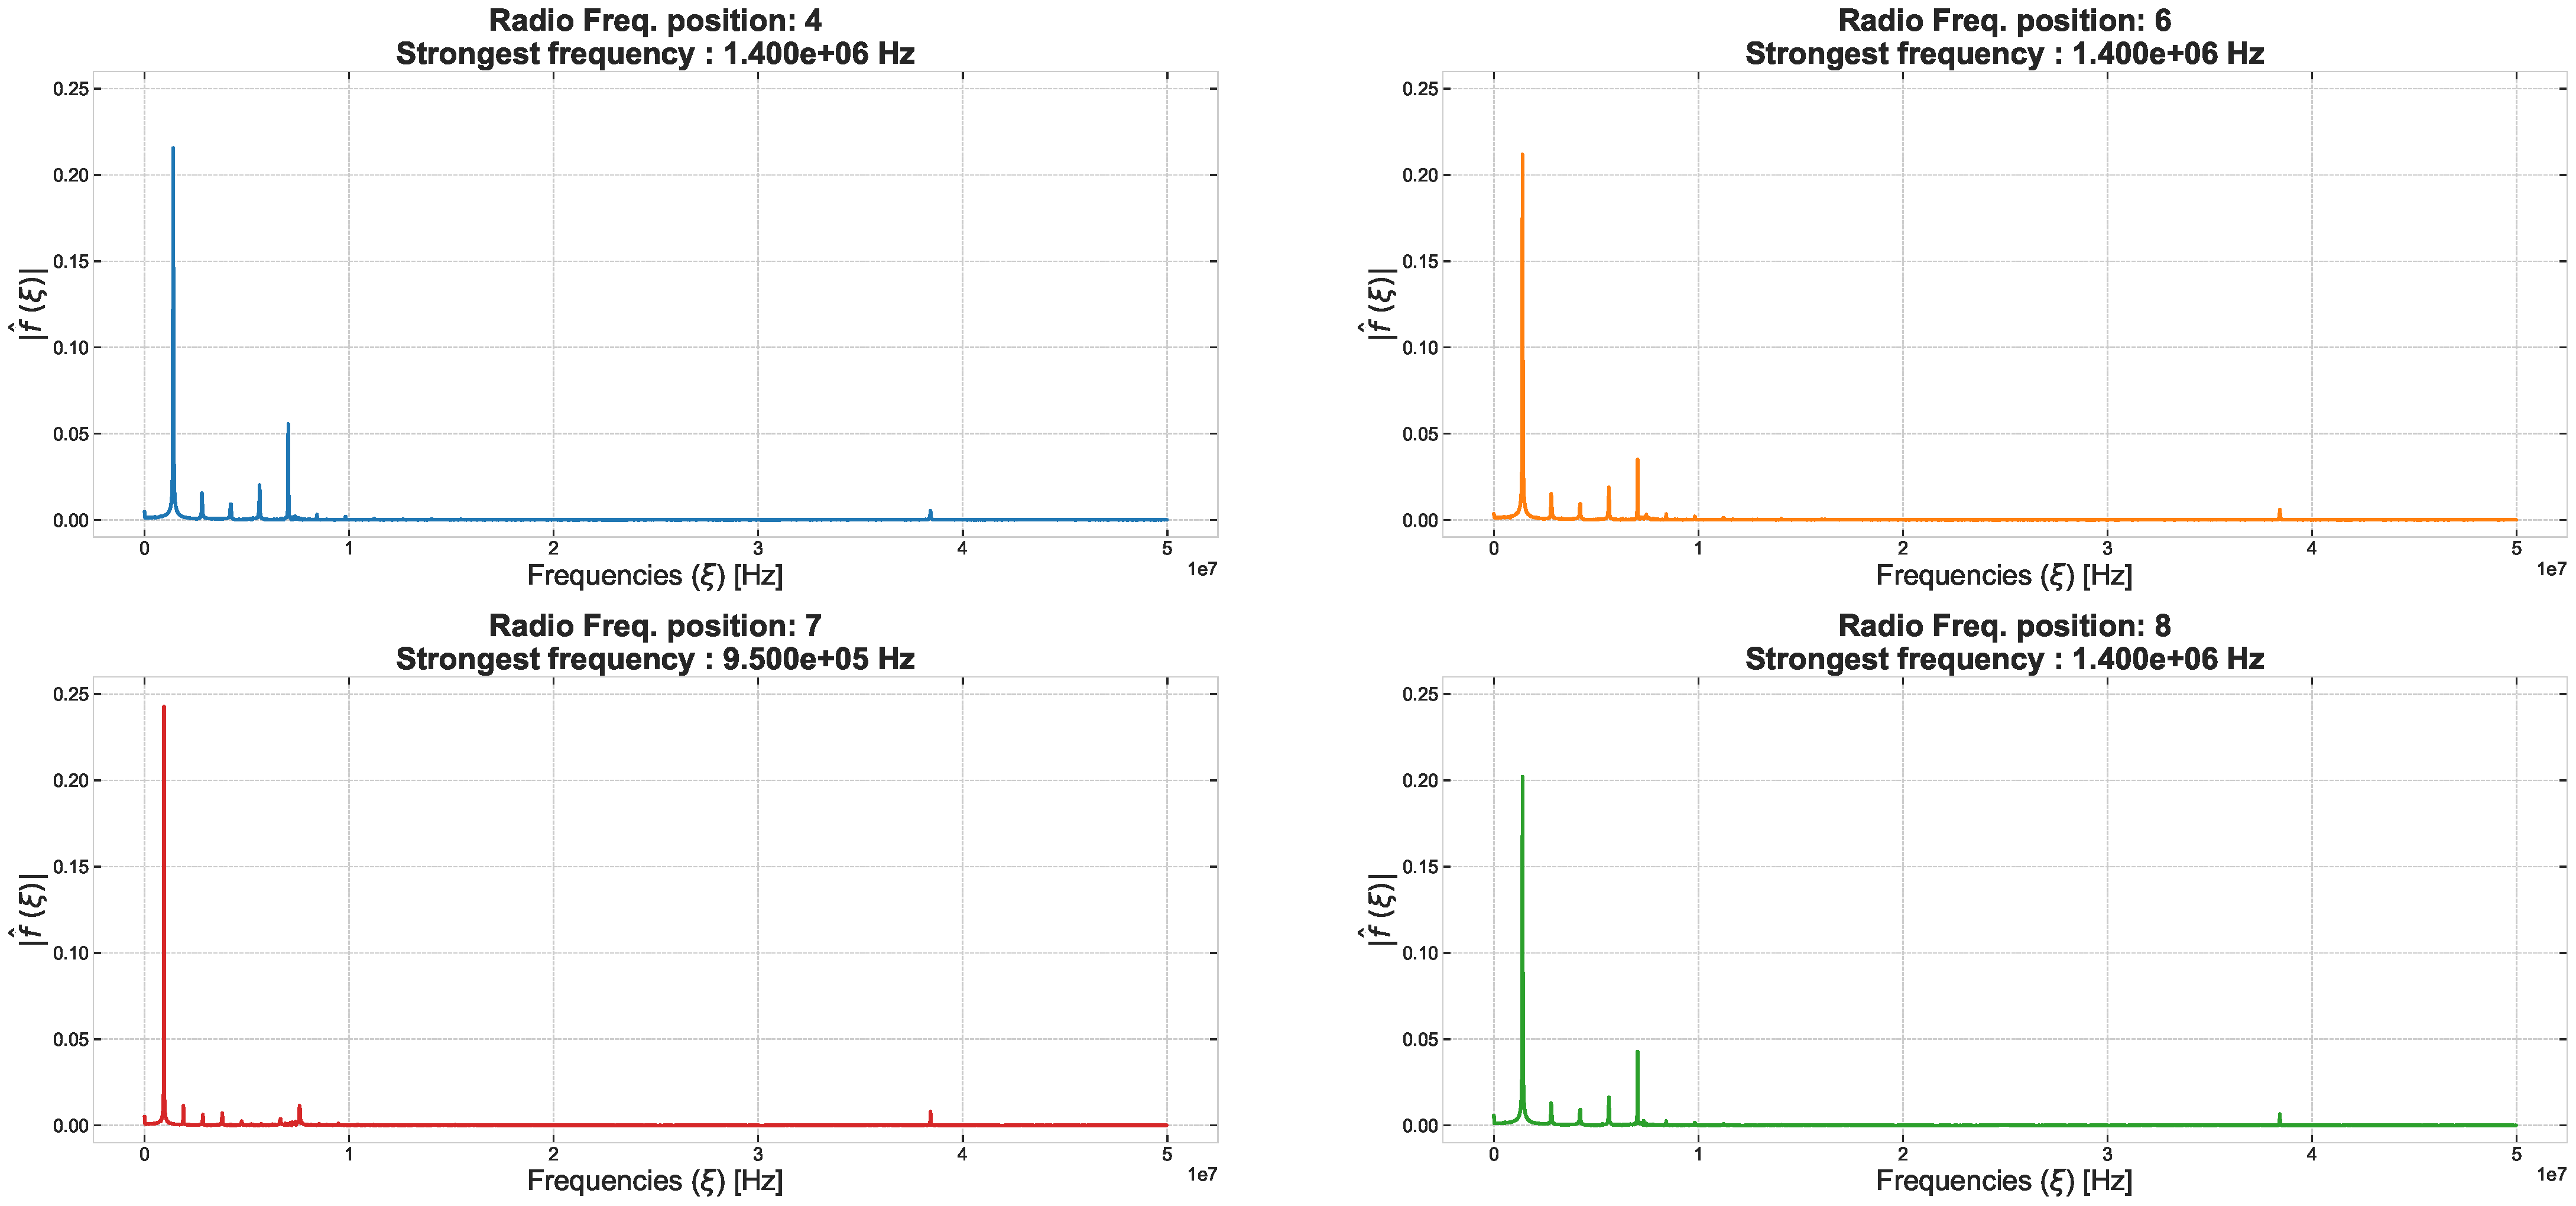
\includegraphics[width=\textwidth]{images/mag_freqs_fourier.pdf}
    \captionof{figure}{A fenti jelek pontos frekvenciáját Fourier-analízissel határoztam meg. Már a labormérés során is problémák adódtak a jelgenerátorral, azonban a vizsgálatukból fény derült a pontos hibára is. A $4$-es, $7$-es és $8$-as állásokban a jeladó pontosan ugyanazon frekvenciákat bocsájtja ki magából, így mérés szempontjából semmilyen különbséggel nem rendelkeznek.} \label{fig:21}
\end{center}
\vspace*{\fill}
\newpage
\topskip0pt
\vspace*{\fill}
\begin{center}
    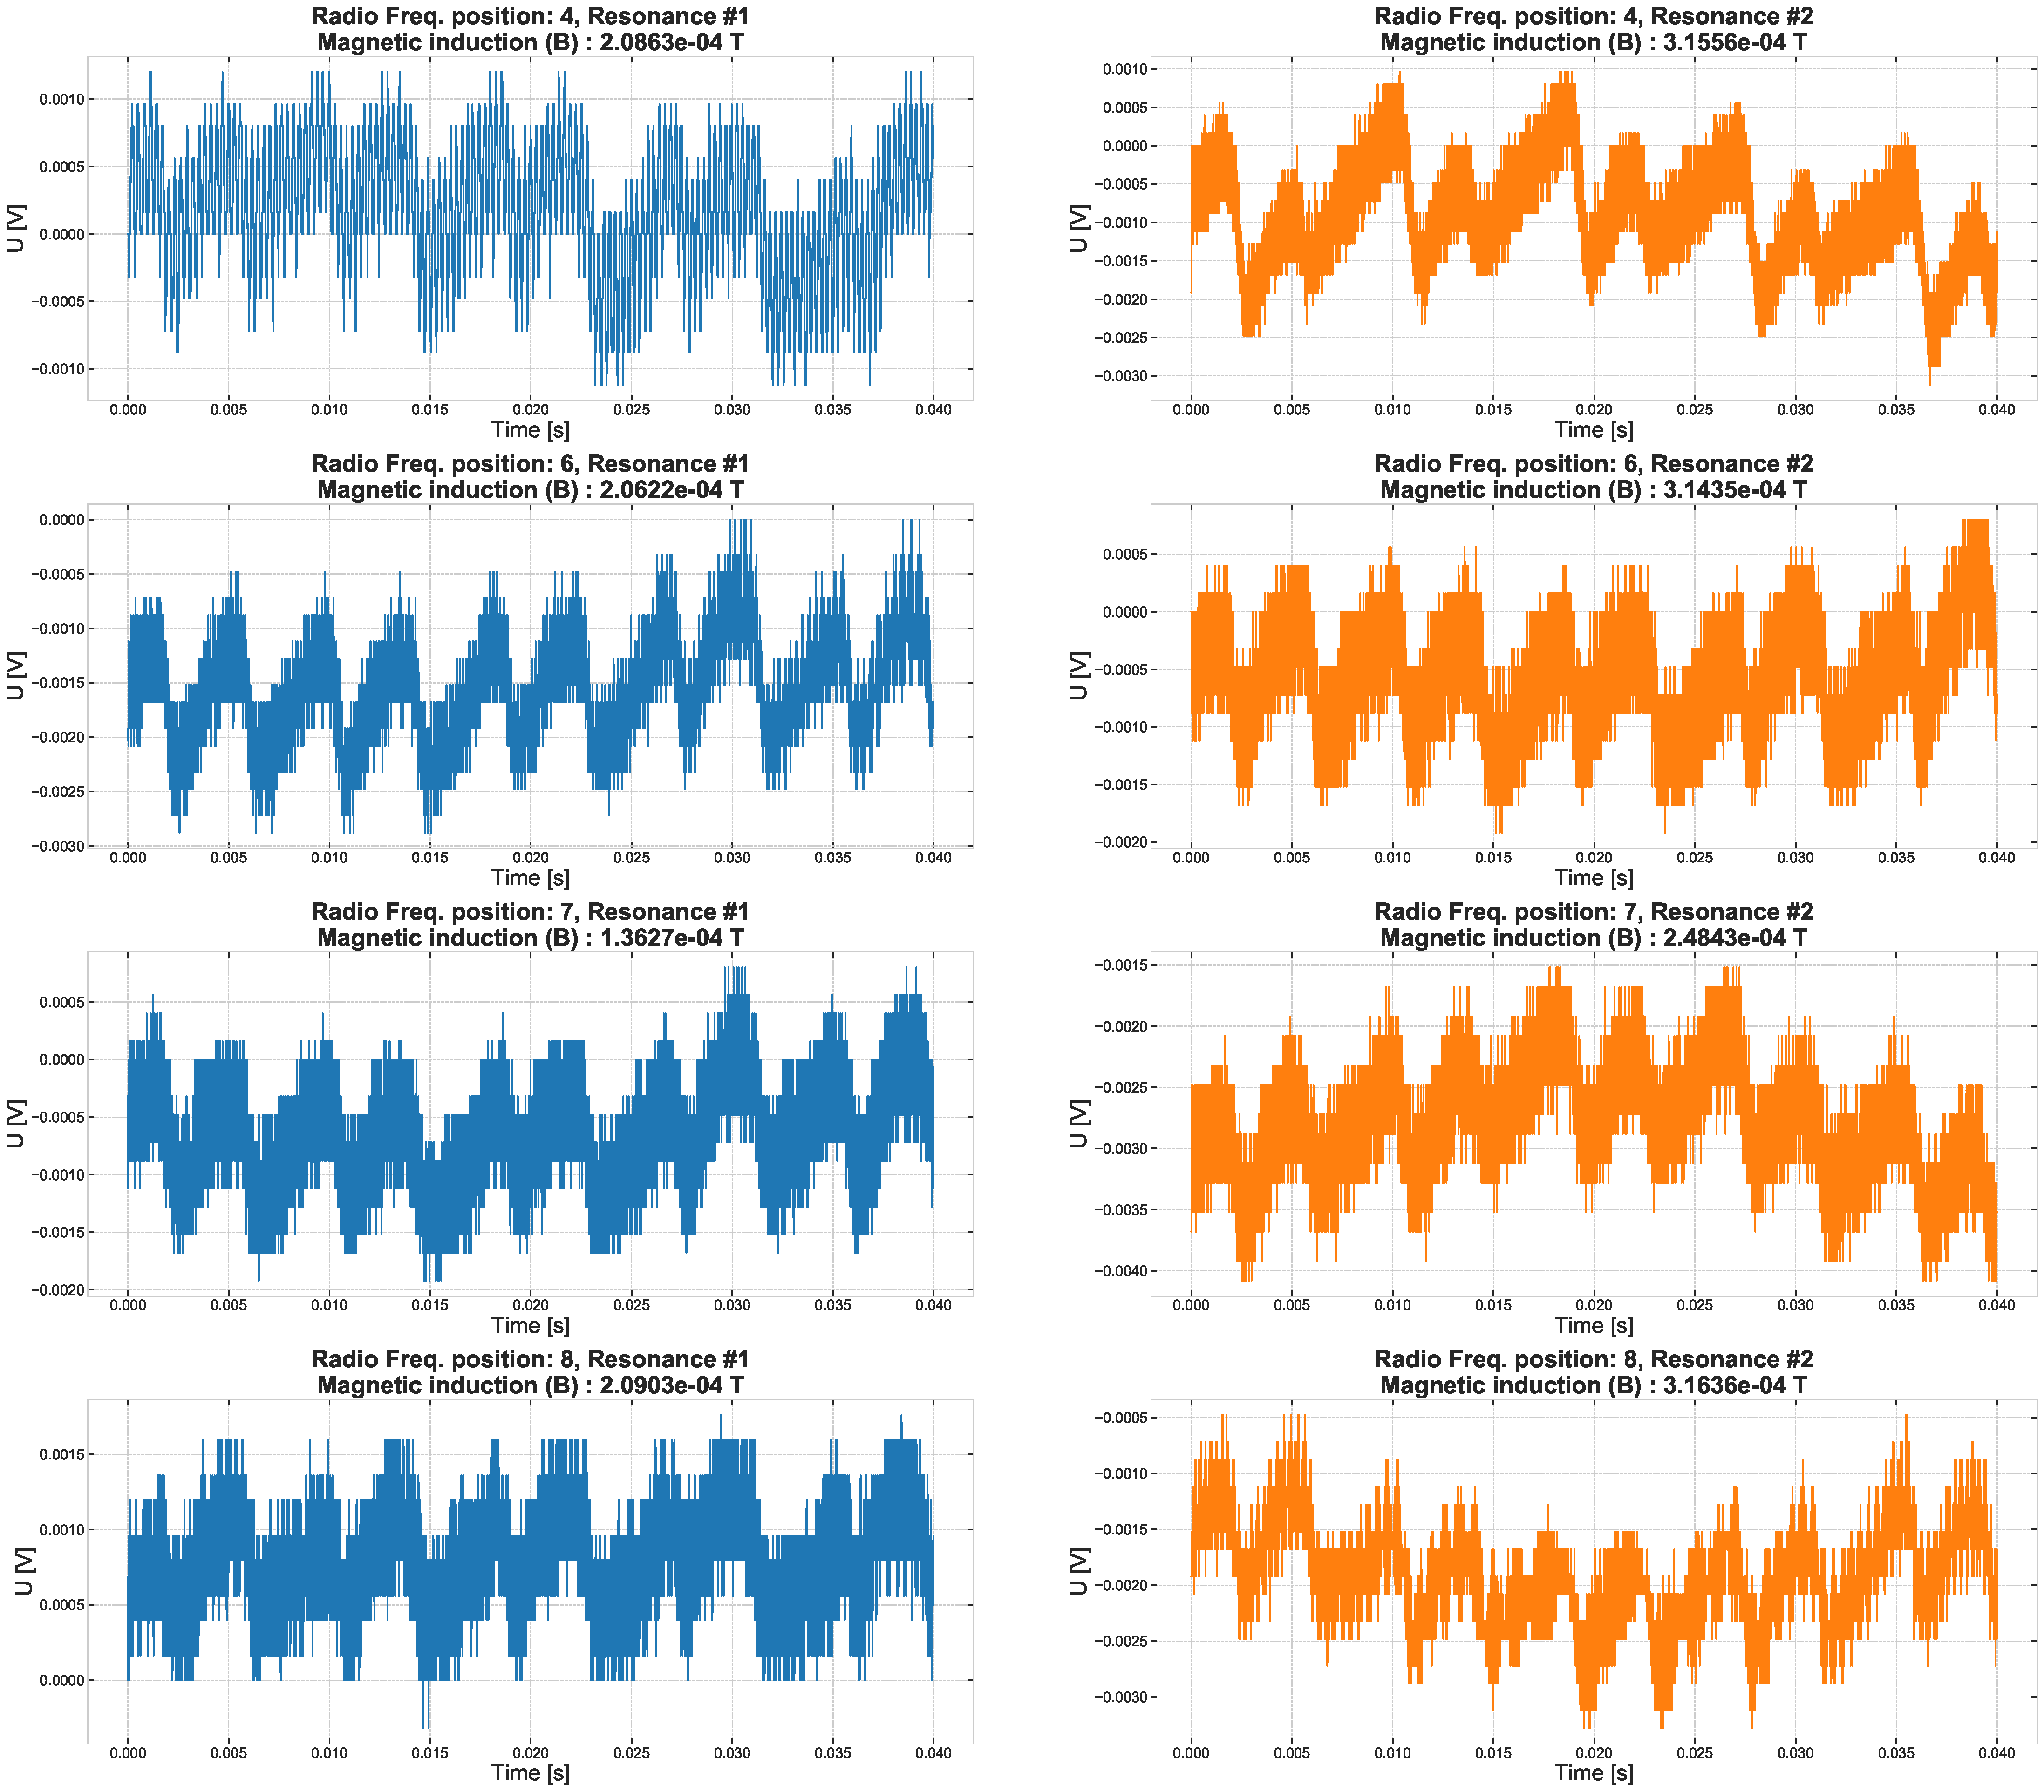
\includegraphics[width=\textwidth]{images/mag_resonance.pdf}
    \captionof{figure}{A $g_{F}$ faktorok meghatározásához kimért $\mu_{B} B^{\ast} = h \nu$ rezonanciákhoz tartozó fotodióda jelalakok a $B_{+}$ polaritás esetében.} \label{fig:22}
\end{center}
\begin{center}
    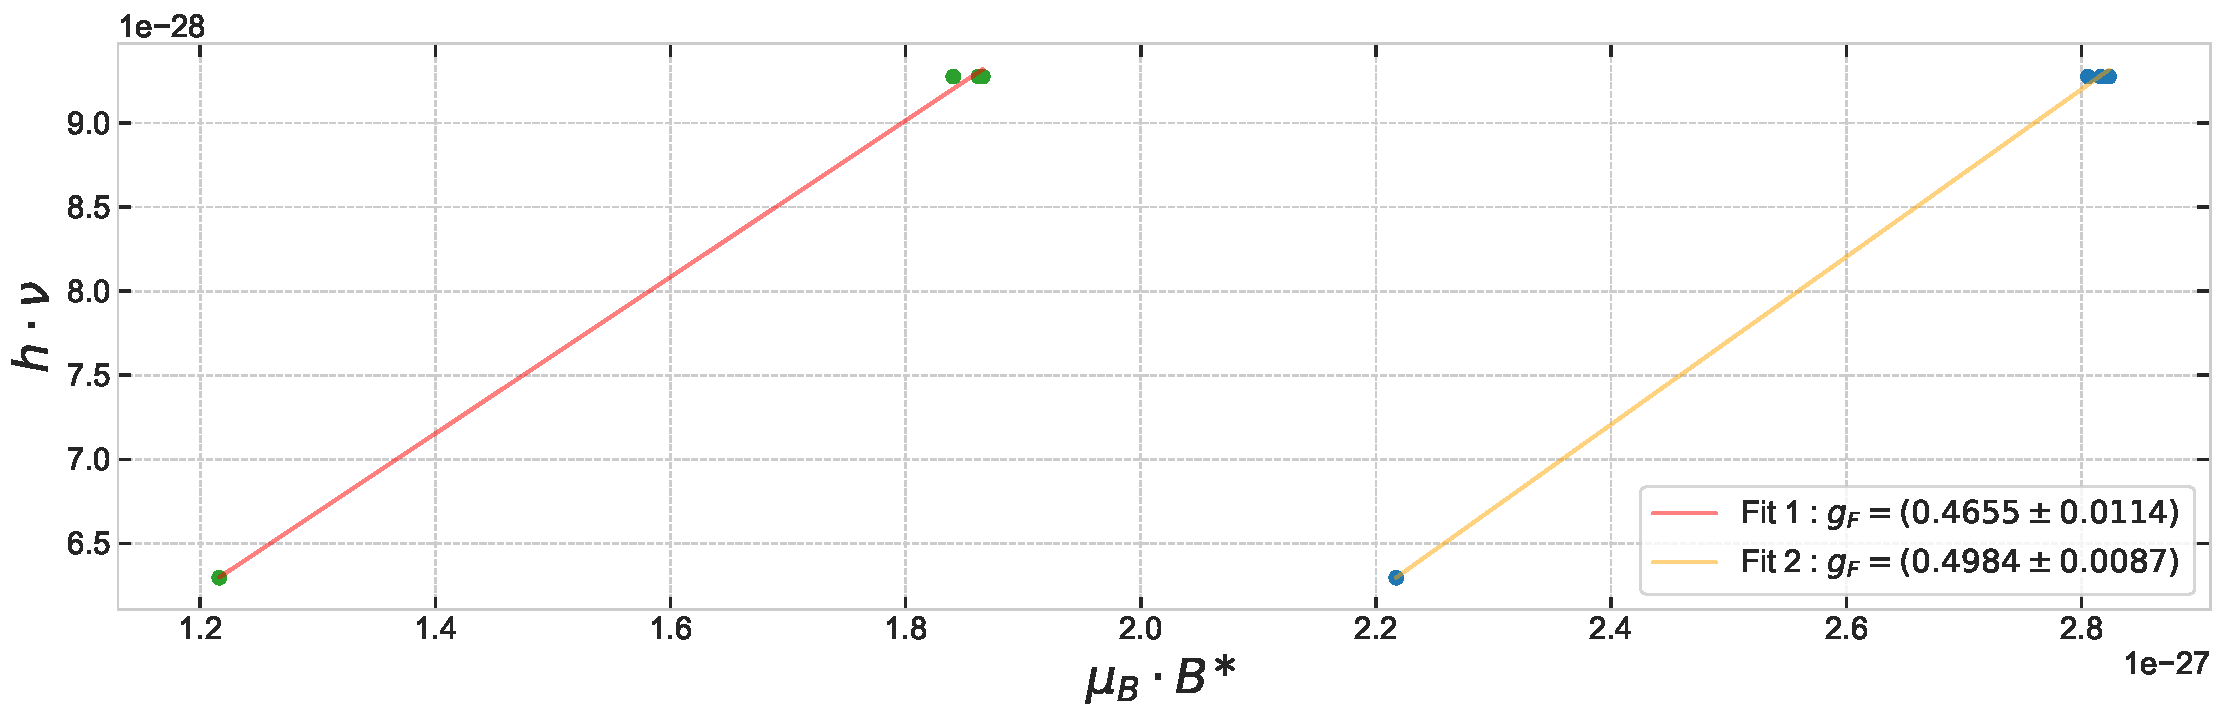
\includegraphics[width=\textwidth]{images/mag_gf_factor.pdf}
    \captionof{figure}{A $g_{F}$ faktorok meghatározásához kimért $\mu_{B} B^{\ast} = h \nu$ rezonanciákra illesztett egyenesek. A mérőműszer hibájából fakadóan csak az $I = 3/2$ magspinű $^{87}$Rb izotópot tudtuk kimutatni, habár a $g_{F} \approx 0,5$ jóval közelebb áll a $^{85}$Rb-höz tartozó értékhez.} \label{fig:23}
\end{center}
\vspace*{\fill}